\documentclass[preprint,
3p]{elsarticle} %review=doublespace preprint=single 5p=2 column
%%% Begin My package additions %%%%%%%%%%%%%%%%%%%

\usepackage[hyphens]{url}

  \journal{Behaviour research and therapy} % Sets Journal name

\usepackage{lineno} % add

\usepackage{graphicx}
%%%%%%%%%%%%%%%% end my additions to header

\usepackage[T1]{fontenc}
\usepackage{lmodern}
\usepackage{amssymb,amsmath}
\usepackage{ifxetex,ifluatex}
\usepackage{fixltx2e} % provides \textsubscript
% use upquote if available, for straight quotes in verbatim environments
\IfFileExists{upquote.sty}{\usepackage{upquote}}{}
\ifnum 0\ifxetex 1\fi\ifluatex 1\fi=0 % if pdftex
  \usepackage[utf8]{inputenc}
\else % if luatex or xelatex
  \usepackage{fontspec}
  \ifxetex
    \usepackage{xltxtra,xunicode}
  \fi
  \defaultfontfeatures{Mapping=tex-text,Scale=MatchLowercase}
  \newcommand{\euro}{€}
\fi
% use microtype if available
\IfFileExists{microtype.sty}{\usepackage{microtype}}{}

\ifxetex
  \usepackage[setpagesize=false, % page size defined by xetex
              unicode=false, % unicode breaks when used with xetex
              xetex]{hyperref}
\else
  \usepackage[unicode=true]{hyperref}
\fi
\hypersetup{breaklinks=true,
            bookmarks=true,
            pdfauthor={},
            pdftitle={Efficacy of Transdiagnostic Cognitive-Behavioral Therapy for Assertiveness: A Randomized Controlled Trial},
            colorlinks=false,
            urlcolor=blue,
            linkcolor=magenta,
            pdfborder={0 0 0}}

\setcounter{secnumdepth}{0}
% Pandoc toggle for numbering sections (defaults to be off)
\setcounter{secnumdepth}{0}


% tightlist command for lists without linebreak
\providecommand{\tightlist}{%
  \setlength{\itemsep}{0pt}\setlength{\parskip}{0pt}}


% Pandoc citation processing
\newlength{\cslhangindent}
\setlength{\cslhangindent}{1.5em}
\newlength{\csllabelwidth}
\setlength{\csllabelwidth}{3em}
\newlength{\cslentryspacingunit} % times entry-spacing
\setlength{\cslentryspacingunit}{\parskip}
% for Pandoc 2.8 to 2.10.1
\newenvironment{cslreferences}%
  {}%
  {\par}
% For Pandoc 2.11+
\newenvironment{CSLReferences}[2] % #1 hanging-ident, #2 entry spacing
 {% don't indent paragraphs
  \setlength{\parindent}{0pt}
  % turn on hanging indent if param 1 is 1
  \ifodd #1
  \let\oldpar\par
  \def\par{\hangindent=\cslhangindent\oldpar}
  \fi
  % set entry spacing
  \setlength{\parskip}{#2\cslentryspacingunit}
 }%
 {}
\usepackage{calc}
\newcommand{\CSLBlock}[1]{#1\hfill\break}
\newcommand{\CSLLeftMargin}[1]{\parbox[t]{\csllabelwidth}{#1}}
\newcommand{\CSLRightInline}[1]{\parbox[t]{\linewidth - \csllabelwidth}{#1}\break}
\newcommand{\CSLIndent}[1]{\hspace{\cslhangindent}#1}

\usepackage{mathptmx}
\usepackage[format=plain,labelsep=period,labelfont=bf,textfont=it]{caption}
\usepackage{booktabs}
\usepackage{longtable}
\usepackage{array}
\usepackage{multirow}
\usepackage{wrapfig}
\usepackage{float}
\usepackage{colortbl}
\usepackage{pdflscape}
\usepackage{tabu}
\usepackage{threeparttable}
\usepackage{threeparttablex}
\usepackage[normalem]{ulem}
\usepackage{makecell}
\usepackage{xcolor}



\begin{document}


\begin{frontmatter}

  \title{Efficacy of Transdiagnostic Cognitive-Behavioral Therapy for
Assertiveness: A Randomized Controlled Trial}
    \author[SU]{Tobias Hagberg%
  %
  }
  
    \author[SU]{Patrik Manhem%
  %
  }
  
    \author[SU]{Martin Oscarsson%
  %
  }
  
    \author[CCI]{Fiona Michel%
  %
  }
  
    \author[LU,KI]{Gerhard Andersson%
  %
  }
  
    \author[SU]{Per Carlbring%
  \corref{cor1}%
  }
   \ead{per.carlbring@psychology.su.se} 
      \affiliation[SU]{Department of Psychology, Stockholm University,
SE-106 91 Stockholm, Sweden}
    \affiliation[KI]{Department of Clinical Neuroscience, Karolinska
Institutet, SE-171 77 Stockholm, Sweden}
    \affiliation[LU]{Department of Behavioural Sciences and Learning,
Department of Biomedical and Clinical Sciences, Linköping University,
SE-581 83 Linköping, Sweden}
    \affiliation[CCI]{Centre for Clinical Interventions, 223 James St,
Northbridge WA 6003, Australia}
    \cortext[cor1]{Corresponding author}
  
  \begin{abstract}
  Assertiveness training has for a long time been an important component
  in cognitive-behavioral therapy (CBT), for example in the treatment of
  social anxiety and in dialectical behavioral therapy. However, the
  assertiveness construct has garnered little attention in recent
  clinical research. The objective of this study was to investigate the
  efficacy of an eight-week transdiagnostic stand-alone internet-based
  CBT intervention, specifically aimed at increasing levels of assertive
  behavior. Following inclusion, we randomized \(N\) = 210 participants
  into three groups: therapist-guided self-help, unguided self-help, and
  a wait-list control condition. After one-year follow-up, we employed a
  linear mixed model to estimate the effects at both posttest and
  follow-up for the primary outcome measures of assertiveness, Adaptive
  and Aggressive Assertiveness Scales, and the Rathus Assertiveness
  Schedule, and secondary outcome measures of anxiety, depression, and
  general well-being. We also assessed reliable clinical change.
  Compared to the wait-list at the post treatment, estimated
  between-group effect sizes on self-rated adaptive assertiveness were
  statistically equivalent for the two treatment groups both at the post
  and at the one-year follow-up time points, ranging from \(ES\) = 0.95
  to \(ES\) = 1.73, with reliable clinical recovery proportions from
  19\% to 36\%. The increase in aggressive assertiveness ranged from
  \(ES\) = --0.62 to \(ES\) = --0.90 compared to the wait-list condition
  at post. For social anxiety symptoms, the effects compared to the
  wait-list at post treatment ranged from \(ES\) = 0.67 to \(ES\) =
  0.93, with reliable clinical recovery from 16\% to 26\%. For
  self-assessed well-being, the effects compared to the wait-list at
  post ranged from \(ES\) = 0.70 to \(ES\) = 1.05. No effects were
  observed for generalized anxiety, although within-group evidence was
  found for a medium effect on depression one year after treatment.
  Overall, the two treatment conditions produced similar effects. In
  general, participation increased healthy assertive expressions
  regardless of treatment condition, thereby reducing self-assessed
  social anxiety, and over time possibly also depression. Participation
  also improved general well-being. The findings demonstrate that the
  assertiveness construct can be a suitable target for intervention,
  with reductions of both psychiatric symptoms and non-syndromal
  problems in daily life. The study was preregistered at
  ClinicalTrials.gov (NCT04240249).
  \end{abstract}
    \begin{keyword}
    assertiveness \sep assertive
behavior \sep anxiety \sep depression \sep stress \sep 
    avoidance
  \end{keyword}
  
 \end{frontmatter}

\hypertarget{introduction}{%
\section{Introduction}\label{introduction}}

Escape and avoidance is associated with the development of maladaptive
behavior among vulnerable participants in laboratory trials (Sheynin et
al., 2014), as well as psychopathologies in clinical presentations.
Experiences of stress, anxiety, and depression are often associated with
avoidance of constructively presenting one's thoughts, feelings, needs,
and wishes in relation to others, that is deficits in assertive behavior
(Speed et al., 2018). Assertiveness can be difficult to delineate from
social skills in general (Linehan, 1979), but a common definition is
``direct, firm, positive {[}\ldots{]} action {[}enabling{]} us to act in
our own best interests, to stand up for ourselves without undue anxiety,
to exercise personal rights without denying the rights of others, and to
express our feelings and needs {[}\ldots{]} honestly and comfortably''
(Alberti and Emmons, 2017, p. 34). Examples include politely saying
``no'' to a boss requesting undue overtime, actively participating in
social activities, accepting/acknowledging a compliment without
deflecting, and verbalizing feelings in personal relationships without
acting out. A lack of assertiveness is associated with several
psychological problems, including stress, generalized anxiety, social
anxiety, depression, and panic disorder, as well as emotional
instability, strained relationships, and low self-esteem (Speed et al.,
2018). While there are diagnoses, diagnostic tools, and treatment
manuals for conditions associated with these problems, no evidence-based
interventions specifically target assertiveness for a broader
population.

Assertiveness training dates back to the very first behavioral therapies
(e.g., Salter, 1949; Wolpe and Lazarus, 1966). In the 1970s, the concept
was popularized in self-help books (e.g., Alberti and Emmons, 1974;
Fensterheim and Baer, 1975; Smith, 1975). Research on assertiveness
training peaked in the 1980s (Speed et al., 2018). Although the
behavioral techniques of the first wave of therapy were supplemented by
cognitive restructuring techniques (e.g., Beck, 1979), in the following
decades, techniques such as modeling and behavior rehearsal remained
active parts of treatments for psychological syndromes such as anxiety
disorders and depression. Linehan's (1979) manual for assertion therapy
combining behavior rehearsal with cognitive restructuring was a stepping
stone toward Dialectical Behavior Therapy (DBT), in which assertion
skills training in a group setting is integral (Linehan, 1993).

Assertion is regarded as a situation-specific trait rather than a
generalized trait (Hull and Hull, 1978). Building on the definition by
Alberti and Emmons (2017), assertiveness can be operationalized as
acting with respect to personal rights without infringing on the rights
of others. Constructive assertion takes into account both the desired
result of the interaction (e.g., saying ``no'' to someone else's demand
or making a request) and the intensity of the interaction, where the
latter is calibrated with regard to both the importance of the
relationship and what Linehan (1993) refers to as self-respect. Using
this definition, assertive behavior can be thought of as the product of
respect for the rights of others and respect for one's own rights. This
definition offers several opportunities for idiographic and contextual
descriptions of assertion in therapy (i.e., when designing in vivo
behavioral experiments, regardless of cultural influences on what is
considered acceptable behavior within a family, community, society,
etc.) (Mitamura, 2018; Sigler et al., 2008).

Speed et al. (2018) concluded that while assertiveness training is part
of DBT, as well as acceptance and commitment therapy (ACT), general
assertiveness training is not often mentioned in the current CBT
literature. Few studies on assertiveness training have been published
since the early 1980s. Recent exceptions include Baker and Jeske (2015),
showing a negative relationship between social anxiety and
assertiveness. Vagos and Pereira (2019) reported a negative association
between mental distress in general and assertiveness, and Antúnez (2020)
found a link between circadian typology and level of assertiveness.
Speed et al. (2018) further concluded that there is potential for
assertiveness training as an intervention for individuals suffering from
anxiety and depression, and as a means to increase relationship
satisfaction. The lack of contemporary evidence for the assertiveness
construct and assertiveness training as a transdiagnostic intervention
calls for new research on the subject.

While the empirical support for assertiveness training is scarce at
best, there is much evidence for the effectiveness of CBT for symptoms
and syndromes associated with inadequate assertiveness. In a review of
meta-analyses, Hofmann et al.~(2012) conclude that CBT is one of the
most effective forms of therapy. This includes its application for
symptoms related to trauma and stress, as well as syndromes related to
depression and anxiety. A review by Andrews et al. (2018) also lends
support to internet-delivered CBT (iCBT) for anxiety and depression,
showing an average between-group effect size of \(g\) = \(0.80\)
compared to the controls. Carlbring et al. (2018) also show that iCBT,
on average, produces equivalent overall effects compared to face-to-face
treatment. iCBT has proven effective in both guided and unguided
applications (i.e., with or without therapist support), although guided
iCBT tends to produce slightly larger effects (Baumeister et al., 2014).
iCBT has also proven effective in transdiagnostic applications,
including interventions targeting stress (Day et al., 2013),
procrastination (Rozental et al., 2015), and perfectionism (Rozental et
al., 2017). The Western Australian Centre for Clinical Interventions
offers various self-help resources for mental health problems. These
resources include Assert Yourself (Michel and Fursland, 2008), a series
of 10 modules with concepts and strategies primarily based on cognitive
behavioral therapy (CBT), with a focus on assertiveness.

This study aimed to conduct a randomized controlled trial (RCT) on the
effects of an eight-week iCBT intervention targeting unhealty
assertiveness, Respekt\textsuperscript{2} (Respect Squared), based on
the Michel and Fursland (2008) modules. We tested the effects on
measures of anxiety, depression, and well-being, as well as the
difference between guided and unguided iCBT against the control group
(three-armed trial).

\hypertarget{method}{%
\section{Method}\label{method}}

\hypertarget{design}{%
\subsection{Design}\label{design}}

We randomly allocated participants to three groups: (1) guided
self-help, (2) unguided self-help, and (3) eight-week wait-list control.
The final sample consisted of 210 participants, with 70 participants per
group. The group sizes were based on an a priori power calculation
according to guidelines for linear models outlined in Cohen (1988),
assuming a between-group effect size of Cohen's \(d\) of \(0.80\) on the
Adaptive and Aggressive Assertiveness Scales (AAA-S; Thompson and
Berenbaum, 2011), power \(.90\), alpha \(.05\), and a \(15\)\% ``worst
case'' drop-out rate per week, with the duration of the intervention
being eight weeks in total.

The study was registered at ClinicalTrials.gov (NCT04240249). An error
in the design was corrected post-registration, in that the Rathus
Assertiveness Schedule (RAS) scale was moved from the secondary outcome
measures category to the primary outcome measures category, as the scale
captures the primary dependent variable of interest. Before recruitment
started, the study received ethical approval from the Swedish Ethical
Review Authority (Diary number: 2019-05165).

\hypertarget{participants}{%
\subsection{Participants}\label{participants}}

Participants were recruited from the public through advertisements on
social media and other websites. Interested individuals were referred to
a purpose-built secure website (Vlaescu et al., 2016) with more
information on the study, including the participation criteria. The
participants were required to be Swedish citizens, at least 18 years of
age, have access to the internet, and be fluent in Swedish. Information
on the website also included the risks associated with participation, as
well as the terms and conditions for participation. Volunteers were
invited to submit their email addresses, and those who did were sent a
link to complete an online screening questionnaire. The questionnaire
included self-report measures of anxiety, depression, general
well-being, and assertiveness, as well as questions regarding
socio-demographics, experiences of psychological treatment, any current
medication, and motivation for participation. See Table 1 for a summary
of the socio-demographic baseline characteristics.

\begin{table}

\caption{\label{tab:demdata}Socio-demographic baseline characteristics of participants.}
\centering
\begin{tabular}[t]{>{\raggedright\arraybackslash}p{10em}>{\centering\arraybackslash}p{4em}>{\centering\arraybackslash}p{4em}>{\centering\arraybackslash}p{4em}>{\centering\arraybackslash}p{4em}}
\toprule
  & Wait-list & Unguided & Guided & Total\\
  & $n$ = 68 & $n$ = 67 & $n$ = 70 & $n$ = 205\\
\midrule
\addlinespace[0.3em]
\multicolumn{5}{l}{Age (years)}\\
\hspace{1em}$M$ ($SD$) & 41 (8) & 41 (9) & 44 (10) & 42 (9)\\
\midrule
\addlinespace[0.3em]
\multicolumn{5}{l}{Sex (\%)}\\
\hspace{1em}Female & 91 & 79 & 93 & 88\\
\midrule
\addlinespace[0.3em]
\multicolumn{5}{l}{Civil status (\%)}\\
\hspace{1em}Single & 37 & 36 & 29 & 34\\
\hspace{1em}Partner & 19 & 25 & 17 & 20\\
\hspace{1em}Married & 37 & 28 & 49 & 38\\
\hspace{1em}Other & 7 & 10 & 6 & 8\\
\midrule
\addlinespace[0.3em]
\multicolumn{5}{l}{Highest educational level (\%)}\\
\hspace{1em}Other & 3 & 1 & 1 & 2\\
\hspace{1em}Middle school & 1 & 0 & 0 & 0\\
\hspace{1em}High school/college & 10 & 9 & 7 & 9\\
\hspace{1em}Vocational training & 7 & 4 & 7 & 6\\
\hspace{1em}Currently at university & 7 & 15 & 10 & 11\\
\hspace{1em}University degree & 71 & 70 & 74 & 72\\
\midrule
\addlinespace[0.3em]
\multicolumn{5}{l}{Occupation (\%)}\\
\hspace{1em}Other & 9 & 6 & 7 & 7\\
\hspace{1em}Student & 7 & 12 & 6 & 8\\
\hspace{1em}Employed & 74 & 76 & 76 & 75\\
\hspace{1em}Unemployed & 4 & 4 & 0 & 3\\
\hspace{1em}Retired & 0 & 0 & 4 & 1\\
\hspace{1em}Parental leave & 0 & 0 & 4 & 1\\
\hspace{1em}Sick leave & 6 & 1 & 3 & 3\\
\midrule
\addlinespace[0.3em]
\multicolumn{5}{l}{Use of psychotropic medications (\%)}\\
\hspace{1em}No & 76 & 70 & 67 & 71\\
\hspace{1em}Yes, previously & 7 & 9 & 17 & 11\\
\hspace{1em}Yes, currently & 16 & 21 & 16 & 18\\
\midrule
\addlinespace[0.3em]
\multicolumn{5}{l}{Previous psychological treatment (\%)}\\
\hspace{1em}No & 38 & 40 & 39 & 39\\
\hspace{1em}Yes & 62 & 60 & 61 & 61\\
\bottomrule
\end{tabular}
\end{table}

In total, 657 individuals submitted their email addresses, of whom 464
completed the screening questionnaire. Of these, 126 were excluded for
meeting the exclusion criteria, which were concurrent psychological
treatment, a recent change in psychotropic medication, lack of time
and/or motivation for participation, and a rating of 15 or above on the
Patient Health Questionnaire (PHQ-9) measure of depression. The
remaining 338 individuals were invited to participate in the study. Of
these, 253 accepted the invitation.

\hypertarget{procedure}{%
\subsection{Procedure}\label{procedure}}

Following the a priori power calculation, 210 participants were
randomized to be included in the study. The remaining 43 individuals
were offered access to the treatment materials but were excluded from
all the analyses. The 210 participants were randomized to the three
treatment conditions. The participants in the guided condition were
randomized to one of two therapists. See Figure 1 for a flow-chart
detailing the recruitment and randomization steps. All randomization was
performed by an independent third party at Stockholm University using
random.org (Haahr, 2018) and sealedenvelope.com (Sealed Envelope Ltd.,
2021).

\hypertarget{measures}{%
\subsection{Measures}\label{measures}}

The data were collected using the measures described below at four time
points: week 0 (pre-treatment), week 4 (during the intervention), week 8
(post-treatment), and at a one-year follow-up. Participants in the
wait-list condition were not included in the follow-up measurement since
they had been given access to the unguided branch of the intervention
after the post-treatment time point.

\hypertarget{primary-measures}{%
\subsubsection{Primary measures}\label{primary-measures}}

Assertiveness style was measured using a Swedish translation
(contributed by TH) of the Adaptive and Aggressive Assertiveness Scales
(AAA-S; Thompson and Berenbaum, 2011), which contains 30 items,
including ``When someone I don't know well borrows something from me and
forgets to return it, I\ldots{} a. Demand it back; b. Ask if she/he is
done and ask for it back'' (a. and b. both scored from 1 = never to 5 =
always). The English-language version of the AAA-S have good internal
consistency for aggressive assertiveness (\(.88\)), and excellent for
adaptive assertiveness (\(.93\)), respectively. A Swedish translation
(contributed by TH) of the Rathus Assertiveness Schedule (RAS; Rathus,
1973) was used as an additional measure of assertiveness style with 30
items, including ``I find it embarrassing to return merchandise'' (+3 =
very characteristic of me, extremely descriptive to --3 = very
uncharacteristic of me, extremely nondescriptive). The RAS has good
internal consistency (\(.87\)) (Thompson and Berenbaum, 2011).

\hypertarget{secondary-measures}{%
\subsubsection{Secondary measures}\label{secondary-measures}}

Depression was measured using the Patient Health Questionnaire 9-Item
Scale (PHQ-9; Kroenke et al., 2010), which contains nine items,
including ``Feeling down, depressed, or hopeless'' (0 = not at all to 3
= nearly every day). Generalized anxiety was measured using the
Generalized Anxiety Disorder 7-item Scale (GAD-7; Spitzer et al., 2006),
which contains seven items, including ``Feeling nervous, anxious, or on
edge'' (0 = not at all to 3 = nearly every day). Social anxiety was
measured using the Liebowitz Social Anxiety Scale (LSAS-SR; Fresco et
al., 2001), which contains 24 items, including ``Calling someone you
don't know very well'' (fear or anxiety, 0 = none to 3 = severe;
avoidance, 0 = never to 3 = usually). General well-being was measured
using the Questionnaire on well-being (Braconier, 2015), which contains
18 items, such as ``To what extent during the past week have you felt
calm and relaxed?'' (0 = never to 5 = very often). These self-report
measures have reported either good or excellent internal consistency
(\(.89\), \(.92\), \(.96\), and \(.93\), respectively).

\hypertarget{intervention}{%
\subsection{Intervention}\label{intervention}}

The intervention was based on the Assert Yourself modules by Michel and
Fursland (2008), which were adapted to Swedish by TH with permission
from the copyright holders. The self-help material teaches the
distinction between different types of assertiveness (constructive,
aggressive, passive, and passive-aggressive). It also aids the reader in
finding reasons to act more assertively and constructively. The material
is inspired by and cites works by Alberti and Emmons (1974), Gambrill
and Richey (1975), and Smith (1975), among others. In the material,
assertiveness is described and operationalized based on Wolpe's (1990)
theoretical assumptions regarding reciprocal inhibition and classic
conditioning: By assertively practicing the expression of feelings,
wishes, and demands in anxiety-evoking situations and relationships,
where the person was previously prone to non-assertive behavior (e.g.,
subdued disappointment or anger), a person may experience less
discomfort from autonomous anxiety responses over time. This is to be
practiced in vivo, not just by acting. The long-term goal is to learn
how to inhibit anxiety by being assertive. In cases where a physical
counterpart is absent and anxiety is invoked by places, objects, or
words, Wolpe (1952) suggests relaxation as a means to inhibit the
anxiety response.

The material also includes a rationale for cognitive restructuring with
methods by Beck (1979), Clark (1986), Clark and Wells (1995), and Powell
(2017). Through behavioral experiments, readers test the validity of
negative thoughts to achieve greater flexibility in their responses.
Furthermore, the material includes a passage on progressive muscle
relaxation for the reader to recognize bodily tension, reduce general
strain, and practice an active coping technique for stressful
situations. Chapters on specific challenges, such as saying ``no,''
dealing with criticism, and coping with disappointment, conclude the
material.

The Swedish adaptation prompted additions to Michel and Fursland (2008),
some of which are presented here. Based on recent research on exposure
and inhibitory learning (e.g., Craske et al., 2008), the participants
were encouraged to actively vary learning situations and work on new
skills in as many environments as possible. In another new passage,
inspired by the works on acceptance by Hayes (e.g., 2004) and others,
the participants were encouraged to actively search for and remain in
the respondent discomfort they previously avoided. In line with Öst's
(2006) recommendations for applied tension, progressive muscle
relaxation was introduced early in the intervention and expanded over
several weeks. The written material was also complemented by
downloadable audio relaxation exercises, videos of conversations and
role-playing, and several new interactive exercises.

Additional support for participants in the guided self-help condition
included weekly messages on the treatment platform, involving feedback
on homework, encouragement, validation, psychoeducation, and answers to
any questions. The therapists were allocated 15 minutes of work per
participant per week.

\hypertarget{therapists}{%
\subsubsection{Therapists}\label{therapists}}

Both therapists working with participants in the guided condition were
final-year clinical psychology students at Stockholm University. Both
had completed basic training in CBT and received continuous supervision
from a licensed psychotherapist with more than two decades of iCBT
experience.

\hypertarget{data-preparation}{%
\subsection{Data preparation}\label{data-preparation}}

Five participants were excluded from the analyses due to wrongful
inclusion, as they were receiving concurrent psychological treatment.

\begin{figure}
\includegraphics[width=1\linewidth]{r2fu-article_files/figure-latex/flowchart-dot-1} \caption{A total of 210 participants were included in the study through randomization and further randomized into three groups: unguided self-help, guided self-help, and wait-list, with 70 participants each.}\label{fig:flowchart-dot}
\end{figure}

\hypertarget{analysis}{%
\subsection{Analysis}\label{analysis}}

All the data were analyzed using R 4.2.2, with the packages lmerTest
(Kuznetsova et al., 2020), emmeans (Lenth, 2020), ggeffects (Lüdecke,
2018), performance (Lüdecke et al., 2022), and clinicalsignificance
(Claus, 2022). All the syntax is available at
https://github.com/hmep/r2fu/, together with the anonymized data.

A linear mixed-effects model was fitted to estimate the fixed effects of
group, time, and group-time interaction, and the random effects of
participant (specifying a random intercept to control for individual
differences), using an unstructured covariance pattern and the
Restricted maximum likelihood (REML) estimation method. The
Kenward-Roger approximations were used to estimate denominator degrees
of freedom. Post-hoc pairwise comparisons of estimated marginal means
were performed using T-tests. The significance of all the post-hoc tests
was decided with Bonferroni-corrected p-values. The proportions of
participants showing reliable change and reaching clinical significance
were determined following Jacobson and Truax (1991), using the ``c''
definition to select the cutoff value. To honor the intention-to-treat
principle in the analysis of clinical significance, the last observation
was carried forward for any missing values.

\begin{figure}
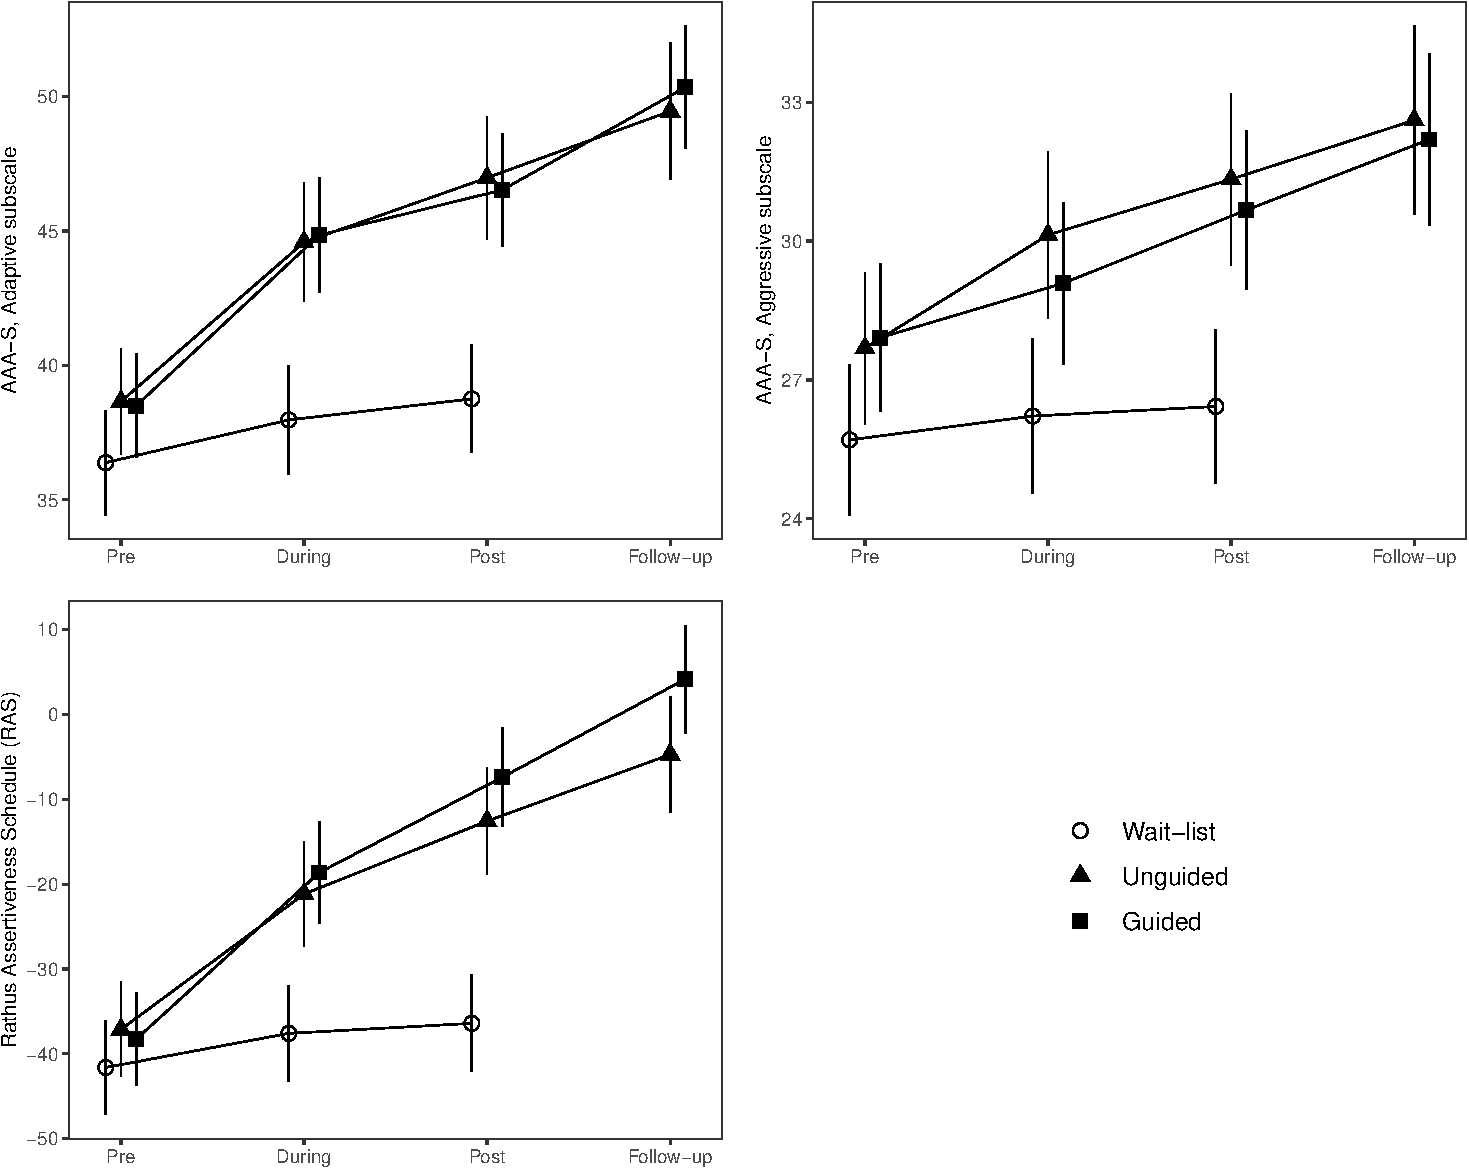
\includegraphics[width=1\linewidth]{r2fu-article_files/figure-latex/emm.primary.plots-1} \caption{Plots of the estimated fixed effects for the primary transdiagnostic scales used to measure skillful, assertive behavior, and aggressive assertive behavior. The participants’ estimated means for all three measures exhibited increasing levels of assertiveness during treatment in the unguided self-help and guided self-help groups, with negligible differences between the two treatment conditions.}\label{fig:emm.primary.plots}
\end{figure}

\begin{figure}
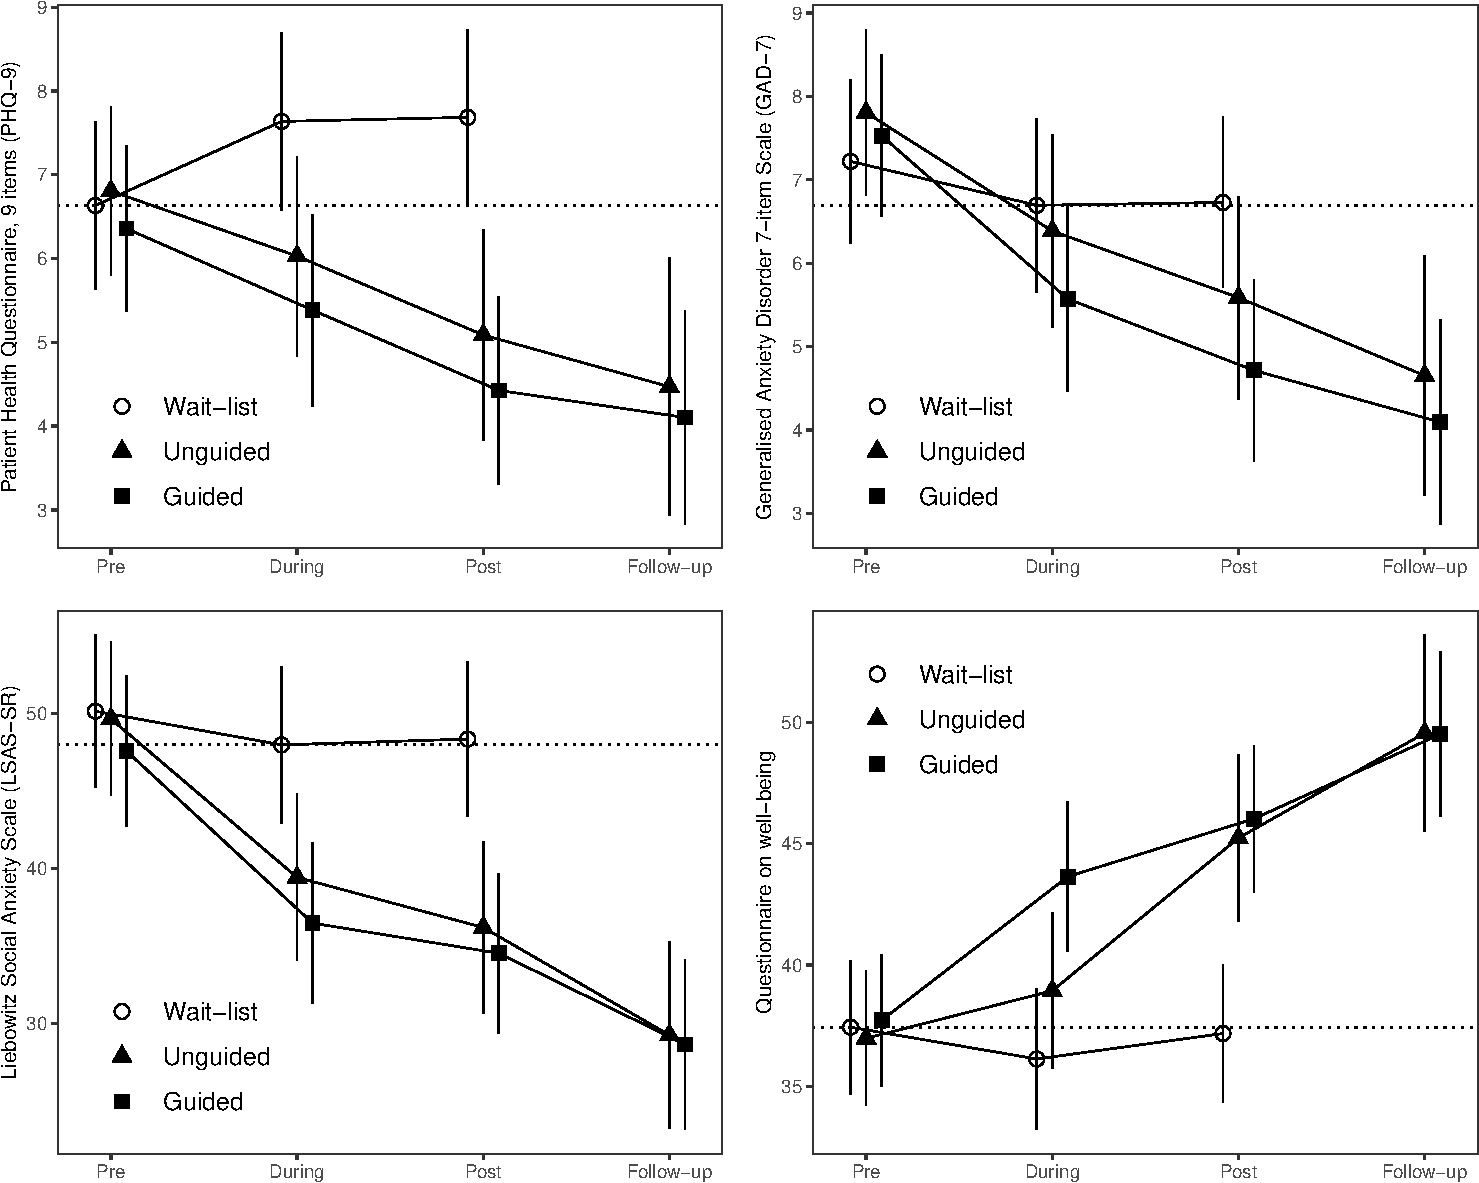
\includegraphics[width=1\linewidth]{r2fu-article_files/figure-latex/emm.secondary.plots-1} \caption{Plots of the estimated fixed effects for the secondary syndromal outcome measures, as well as for the general well-being measure. Participation in the unguided self-help and guided self-help conditions led to significant symptom alleviation between the pre and post time points as well as between the pre and one-year follow-up time points for depression and social anxiety. Participation in both treatment groups also led to significant increases in well-being. As with the transdiagnostic measures of assertive behavior, the differences between the post and follow-up time points were statistically inappreciable for all measures, in both treatment groups. The wait-list control group did not significantly change between any time points for either measure. However, to stay on the conservative side and counteract even the slightest nocebo effect of the wait-list condition, the most conservative estimate for the wait-list control condition was used in each follow-up between-group comparison; see the dotted line for a visual representation of the selected time point.}\label{fig:emm.secondary.plots}
\end{figure}

\begin{table}

\caption{\label{tab:effsizetab}Within-group effect sizes [95\% CI] comparing estimated marginal means between Pre- and Post-treatment, as well as between Pre-treatment and 1-year Follow-up, and between group effect sizes [95\% CI] at Post-treatment and 1-year Follow-up.}
\centering
\fontsize{4}{6}\selectfont
\begin{threeparttable}
\begin{tabular}[t]{>{\raggedleft\arraybackslash}p{19em}>{\raggedright\arraybackslash}p{10.5em}>{\raggedright\arraybackslash}p{11em}>{\raggedright\arraybackslash}p{10.5em}>{\raggedright\arraybackslash}p{10.5em}>{\raggedright\arraybackslash}p{10.5em}>{\raggedright\arraybackslash}p{10.5em}l}
\toprule
\multicolumn{1}{c}{ } & \multicolumn{3}{c}{Primary transdiagnostic measures of skillful behavior} & \multicolumn{4}{c}{Secondary measures of syndromal symptoms and well-being} \\
\cmidrule(l{3pt}r{3pt}){2-4} \cmidrule(l{3pt}r{3pt}){5-8}
  & \parbox{10.5em}{\hfil{}\hspace{2em}AAA-S Adaptive\hfil{}} & \parbox{10.5em}{\hfil{}\hspace{2em}AAA-S Aggressive\hfil{}} & \parbox{10.5em}{\hfil{}\hspace{2em}RAS\hfil{}} & \parbox{10.5em}{\hfil{}\hspace{2em}PHQ-9\hfil{}} & \parbox{10.5em}{\hfil{}\hspace{2em}GAD-7\hfil{}} & \parbox{10.5em}{\hfil{}\hspace{2em}LSAS-SR\hfil{}} & \parbox{10.5em}{\hfil{}\hspace{2em}Well-being\hfil{}}\\
\midrule
\addlinespace[0.3em]
\multicolumn{8}{l}{Within-group effect sizes}\\
\hspace{1em}Unguided, Pre vs. Post & \parbox[b]{4.25em}{\flushright$1.01$}~[$0.76$, $1.26$]\hbox to 0bp{\textsuperscript{***}} & \parbox[b]{4.25em}{\flushright$-0.53$}~[$-0.75$, $-0.31$]\hbox to 0bp{\textsuperscript{***}} & \parbox[b]{4.25em}{\flushright$1.05$}~[$0.82$, $1.28$]\hbox to 0bp{\textsuperscript{***}} & \parbox[b]{4.25em}{\flushright$0.41$}~[$0.10$, $0.71$] & \parbox[b]{4.25em}{\flushright$0.53$}~[$0.25$, $0.82$]\hbox to 0bp{\textsuperscript{*}} & \parbox[b]{4.25em}{\flushright$0.65$}~[$0.45$, $0.84$]\hbox to 0bp{\textsuperscript{***}} & \parbox[b]{4.25em}{\flushright$0.71$}~[$0.42$, $1.00$]\hbox to 0bp{\textsuperscript{***}}\\
\hspace{1em}Unguided, Pre vs. Follow-up & \parbox[b]{4.25em}{\flushright$1.31$}~[$1.02$, $1.60$]\hbox to 0bp{\textsuperscript{***}} & \parbox[b]{4.25em}{\flushright$-0.72$}~[$-0.97$, $-0.47$]\hbox to 0bp{\textsuperscript{***}} & \parbox[b]{4.25em}{\flushright$1.39$}~[$1.12$, $1.65$]\hbox to 0bp{\textsuperscript{***}} & \parbox[b]{4.25em}{\flushright$0.55$}~[$0.18$, $0.92$] & \parbox[b]{4.25em}{\flushright$0.76$}~[$0.42$, $1.10$]\hbox to 0bp{\textsuperscript{***}} & \parbox[b]{4.25em}{\flushright$0.98$}~[$0.75$, $1.21$]\hbox to 0bp{\textsuperscript{***}} & \parbox[b]{4.25em}{\flushright$1.09$}~[$0.74$, $1.43$]\hbox to 0bp{\textsuperscript{***}}\\
\hspace{1em}Unguided, Post vs. Follow-up & \parbox[b]{4.25em}{\flushright$0.30$}~[$0.00$, $0.60$] & \parbox[b]{4.25em}{\flushright$-0.19$}~[$-0.45$, $0.08$] & \parbox[b]{4.25em}{\flushright$0.34$}~[$0.07$, $0.60$] & \parbox[b]{4.25em}{\flushright$0.15$}~[$-0.25$, $0.54$] & \parbox[b]{4.25em}{\flushright$0.23$}~[$-0.14$, $0.59$] & \parbox[b]{4.25em}{\flushright$0.33$}~[$0.10$, $0.57$] & \parbox[b]{4.25em}{\flushright$0.37$}~[$0.01$, $0.74$]\\
\midrule
\hspace{1em}Guided, Pre vs. Post & \parbox[b]{4.25em}{\flushright$0.98$}~[$0.75$, $1.20$]\hbox to 0bp{\textsuperscript{***}} & \parbox[b]{4.25em}{\flushright$-0.40$}~[$-0.60$, $-0.21$]\hbox to 0bp{\textsuperscript{**}} & \parbox[b]{4.25em}{\flushright$1.32$}~[$1.11$, $1.53$]\hbox to 0bp{\textsuperscript{***}} & \parbox[b]{4.25em}{\flushright$0.46$}~[$0.18$, $0.73$] & \parbox[b]{4.25em}{\flushright$0.68$}~[$0.42$, $0.93$]\hbox to 0bp{\textsuperscript{***}} & \parbox[b]{4.25em}{\flushright$0.63$}~[$0.46$, $0.80$]\hbox to 0bp{\textsuperscript{***}} & \parbox[b]{4.25em}{\flushright$0.72$}~[$0.46$, $0.97$]\hbox to 0bp{\textsuperscript{***}}\\
\hspace{1em}Guided, Pre vs. Follow-up & \parbox[b]{4.25em}{\flushright$1.44$}~[$1.18$, $1.70$]\hbox to 0bp{\textsuperscript{***}} & \parbox[b]{4.25em}{\flushright$-0.63$}~[$-0.85$, $-0.40$]\hbox to 0bp{\textsuperscript{***}} & \parbox[b]{4.25em}{\flushright$1.81$}~[$1.57$, $2.05$]\hbox to 0bp{\textsuperscript{***}} & \parbox[b]{4.25em}{\flushright$0.53$}~[$0.23$, $0.84$]\hbox to 0bp{\textsuperscript{*}} & \parbox[b]{4.25em}{\flushright$0.83$}~[$0.53$, $1.12$]\hbox to 0bp{\textsuperscript{***}} & \parbox[b]{4.25em}{\flushright$0.91$}~[$0.71$, $1.11$]\hbox to 0bp{\textsuperscript{***}} & \parbox[b]{4.25em}{\flushright$1.02$}~[$0.73$, $1.31$]\hbox to 0bp{\textsuperscript{***}}\\
\hspace{1em}Guided, Post vs. Follow-up & \parbox[b]{4.25em}{\flushright$0.46$}~[$0.21$, $0.72$]\hbox to 0bp{\textsuperscript{*}} & \parbox[b]{4.25em}{\flushright$-0.22$}~[$-0.45$, $0.00$] & \parbox[b]{4.25em}{\flushright$0.49$}~[$0.26$, $0.73$]\hbox to 0bp{\textsuperscript{**}} & \parbox[b]{4.25em}{\flushright$0.08$}~[$-0.24$, $0.40$] & \parbox[b]{4.25em}{\flushright$0.15$}~[$-0.15$, $0.45$] & \parbox[b]{4.25em}{\flushright$0.28$}~[$0.09$, $0.48$] & \parbox[b]{4.25em}{\flushright$0.30$}~[$0.01$, $0.59$]\\
\midrule
\hspace{1em}Wait-list, Pre vs. Post & \parbox[b]{4.25em}{\flushright$0.29$}~[$0.09$, $0.49$] & \parbox[b]{4.25em}{\flushright$-0.11$}~[$-0.29$, $0.07$] & \parbox[b]{4.25em}{\flushright$0.22$}~[$0.03$, $0.41$] & \parbox[b]{4.25em}{\flushright$-0.25$}~[$-0.50$, $0.01$] & \parbox[b]{4.25em}{\flushright$0.12$}~[$-0.12$, $0.36$] & \parbox[b]{4.25em}{\flushright$0.09$}~[$-0.07$, $0.24$] & \parbox[b]{4.25em}{\flushright$-0.02$}~[$-0.25$, $0.21$]\\
\midrule
\addlinespace[0.3em]
\multicolumn{8}{l}{Between-group effect sizes}\\
\hspace{1em}Unguided at Post vs. Wait-list at Post & \parbox[b]{4.25em}{\flushright$1.00$}~[$0.62$, $1.38$]\hbox to 0bp{\textsuperscript{***}} & \parbox[b]{4.25em}{\flushright$-0.72$}~[$-1.09$, $-0.35$]\hbox to 0bp{\textsuperscript{**}} & \parbox[b]{4.25em}{\flushright$1.02$}~[$0.65$, $1.39$]\hbox to 0bp{\textsuperscript{***}} & \parbox[b]{4.25em}{\flushright$0.61$}~[$0.22$, $1.01$] & \parbox[b]{4.25em}{\flushright$0.27$}~[$-0.11$, $0.66$] & \parbox[b]{4.25em}{\flushright$0.59$}~[$0.22$, $0.95$] & \parbox[b]{4.25em}{\flushright$0.70$}~[$0.31$, $1.08$]\hbox to 0bp{\textsuperscript{*}}\\
\hspace{1em}Unguided at Follow-up vs. Wait-list at Post & \parbox[b]{4.25em}{\flushright$1.30$}~[$0.90$, $1.71$]\hbox to 0bp{\textsuperscript{***}} & \parbox[b]{4.25em}{\flushright$-0.90$}~[$-1.29$, $-0.51$]\hbox to 0bp{\textsuperscript{***}} & \parbox[b]{4.25em}{\flushright$1.35$}~[$0.96$, $1.75$]\hbox to 0bp{\textsuperscript{***}} & \parbox[b]{4.25em}{\flushright$0.76$}~[$0.32$, $1.20$]\hbox to 0bp{\textsuperscript{*}} & \parbox[b]{4.25em}{\flushright$0.50$}~[$0.07$, $0.93$] & \parbox[b]{4.25em}{\flushright$0.92$}~[$0.54$, $1.30$]\hbox to 0bp{\textsuperscript{***}} & \parbox[b]{4.25em}{\flushright$1.07$}~[$0.63$, $1.50$]\hbox to 0bp{\textsuperscript{***}}\\
\hspace{1em}Unguided at Follow-up vs. Wait-list at \dag & \parbox{10.5em}{\hfil{}(idem)\hfil{}} & \parbox{10.5em}{\hfil{}(idem)\hfil{}} & \parbox{10.5em}{\hfil{}(idem)\hfil{}} & \parbox[b]{4.25em}{\flushright$0.51$}~[$0.07$, $0.95$] & \parbox[b]{4.25em}{\flushright$0.49$}~[$0.06$, $0.92$] & \parbox[b]{4.25em}{\flushright$0.90$}~[$0.52$, $1.29$]\hbox to 0bp{\textsuperscript{***}} & \parbox[b]{4.25em}{\flushright$1.05$}~[$0.62$, $1.47$]\hbox to 0bp{\textsuperscript{***}}\\
\midrule
\hspace{1em}Guided at Post vs. Wait-list at Post & \parbox[b]{4.25em}{\flushright$0.95$}~[$0.59$, $1.30$]\hbox to 0bp{\textsuperscript{***}} & \parbox[b]{4.25em}{\flushright$-0.62$}~[$-0.97$, $-0.27$]\hbox to 0bp{\textsuperscript{*}} & \parbox[b]{4.25em}{\flushright$1.24$}~[$0.88$, $1.60$]\hbox to 0bp{\textsuperscript{***}} & \parbox[b]{4.25em}{\flushright$0.77$}~[$0.40$, $1.14$]\hbox to 0bp{\textsuperscript{**}} & \parbox[b]{4.25em}{\flushright$0.48$}~[$0.12$, $0.85$] & \parbox[b]{4.25em}{\flushright$0.67$}~[$0.32$, $1.02$]\hbox to 0bp{\textsuperscript{*}} & \parbox[b]{4.25em}{\flushright$0.76$}~[$0.40$, $1.13$]\hbox to 0bp{\textsuperscript{**}}\\
\hspace{1em}Guided at Follow-up vs. Wait-list at Post & \parbox[b]{4.25em}{\flushright$1.41$}~[$1.03$, $1.79$]\hbox to 0bp{\textsuperscript{***}} & \parbox[b]{4.25em}{\flushright$-0.84$}~[$-1.21$, $-0.47$]\hbox to 0bp{\textsuperscript{***}} & \parbox[b]{4.25em}{\flushright$1.73$}~[$1.36$, $2.11$]\hbox to 0bp{\textsuperscript{***}} & \parbox[b]{4.25em}{\flushright$0.85$}~[$0.45$, $1.24$]\hbox to 0bp{\textsuperscript{**}} & \parbox[b]{4.25em}{\flushright$0.63$}~[$0.25$, $1.02$] & \parbox[b]{4.25em}{\flushright$0.95$}~[$0.58$, $1.31$]\hbox to 0bp{\textsuperscript{***}} & \parbox[b]{4.25em}{\flushright$1.06$}~[$0.67$, $1.45$]\hbox to 0bp{\textsuperscript{***}}\\
\hspace{1em}Guided at Follow-up vs. Wait-list at \dag & \parbox{10.5em}{\hfil{}(idem)\hfil{}} & \parbox{10.5em}{\hfil{}(idem)\hfil{}} & \parbox{10.5em}{\hfil{}(idem)\hfil{}} & \parbox[b]{4.25em}{\flushright$0.60$}~[$0.21$, $0.98$] & \parbox[b]{4.25em}{\flushright$0.63$}~[$0.24$, $1.02$] & \parbox[b]{4.25em}{\flushright$0.93$}~[$0.57$, $1.30$]\hbox to 0bp{\textsuperscript{***}} & \parbox[b]{4.25em}{\flushright$1.04$}~[$0.66$, $1.43$]\hbox to 0bp{\textsuperscript{***}}\\
\midrule
\hspace{1em}Guided vs. Unguided at Post & \parbox[b]{4.25em}{\flushright$-0.05$}~[$-0.43$, $0.32$] & \parbox[b]{4.25em}{\flushright$0.10$}~[$-0.27$, $0.47$] & \parbox[b]{4.25em}{\flushright$0.22$}~[$-0.15$, $0.59$] & \parbox[b]{4.25em}{\flushright$0.16$}~[$-0.24$, $0.56$] & \parbox[b]{4.25em}{\flushright$0.21$}~[$-0.18$, $0.60$] & \parbox[b]{4.25em}{\flushright$0.08$}~[$-0.29$, $0.45$] & \parbox[b]{4.25em}{\flushright$0.07$}~[$-0.33$, $0.47$]\\
\hspace{1em}Guided vs. Unguided at Follow-up & \parbox[b]{4.25em}{\flushright$0.11$}~[$-0.31$, $0.53$] & \parbox[b]{4.25em}{\flushright$0.06$}~[$-0.34$, $0.46$] & \parbox[b]{4.25em}{\flushright$0.38$}~[$-0.02$, $0.78$] & \parbox[b]{4.25em}{\flushright$0.09$}~[$-0.39$, $0.56$] & \parbox[b]{4.25em}{\flushright$0.13$}~[$-0.32$, $0.59$] & \parbox[b]{4.25em}{\flushright$0.03$}~[$-0.37$, $0.42$] & \parbox[b]{4.25em}{\flushright$-0.00$}~[$-0.46$, $0.45$]\\
\bottomrule
\end{tabular}
\begin{tablenotes}
\item \textit{Notes.} 
\item CI = confidence interval
\item AAA-S Adaptive = Adaptive and Aggressive Assertiveness Scales, Adaptive subscale; AAA-S Aggressive = Adaptive and Aggressive Assertiveness Scales, Aggressive Subscale, RAS = Rathus Assertiveness Schedule; PHQ-9 = Patient Health Questionnaire, 9 items; GAD-7 = Generalised Anxiety Disorder 7-item Scale; LSAS-SR = Liebowitz Social Anxiety Scale; Well-being = Questionnaire on Well-being.
\item Pre = pre-treatment measurement at 0 weeks; During = measurement during week 4; Post = measurement after completion of treatment at week 8; Follow-up = measurement at 1 year after completion.
\item \textsuperscript{\dag} = the most conservative measurement for the Wait-list control condition, in order to suppress any nocebo effects; see dotted lines in graphs in Figure 3 for identification of time point.
\item \textsuperscript{*} = \textit{p} < .05, \textsuperscript{**} = \textit{p} < .01, \textsuperscript{***} = \textit{p} < .00; \textit{p}-values are Bonferroni adjusted, based on pairwise comparisons of all sampled time points and conditions.
\end{tablenotes}
\end{threeparttable}
\end{table}

\begin{table}

\caption{\label{tab:clinsigtab}Clinical significance summary of the number (and proportion in \%) of participants that changed reliably and moved from the clinical to the functional population from Pre-treatment to Post- and 1-year Follow-up-time points respectively (rows named 'Recovered'). For missing values (i.e., caused by drop-outs), the last collected value was moved forward to the next measurement time point, in order to respect the intention to treat principle.}
\centering
\fontsize{8}{10}\selectfont
\begin{threeparttable}
\begin{tabular}[t]{>{\raggedleft\arraybackslash}p{7em}>{\raggedright\arraybackslash}p{7em}>{\raggedright\arraybackslash}p{7em}>{\raggedright\arraybackslash}p{7em}>{\raggedright\arraybackslash}p{7em}>{\raggedright\arraybackslash}p{7em}}
\toprule
\multicolumn{1}{c}{ } & \multicolumn{1}{c}{Wait-list} & \multicolumn{2}{c}{Unguided self-help} & \multicolumn{2}{c}{Guided self-help} \\
\cmidrule(l{3pt}r{3pt}){2-2} \cmidrule(l{3pt}r{3pt}){3-4} \cmidrule(l{3pt}r{3pt}){5-6}
  & \parbox{7em}{\hfil{}Pre--Post\hfil{}} & \parbox{7em}{\hfil{}Pre--Post\hfil{}} & \parbox{7em}{\hfil{}Pre--Follow-up\hfil{}} & \parbox{7em}{\hfil{}Pre--Post\hfil{}} & \parbox{7em}{\hfil{}Pre--Follow-up\hfil{}}\\
\midrule
\addlinespace[0.3em]
\multicolumn{6}{l}{AAA-S Adaptive}\\
\hspace{1em}Recovered & \hskip -.5em\parbox[b]{3.12em}{\flushright$3$} ($4$\%) & \hskip -.5em\parbox[b]{3.12em}{\flushright$13$} ($19$\%)\hbox to 0bp{\textsuperscript{*}} & \hskip -.5em\parbox[b]{3.12em}{\flushright$15$} ($22$\%)\hbox to 0bp{\textsuperscript{*}} & \hskip -.5em\parbox[b]{3.12em}{\flushright$13$} ($19$\%) & \hskip -.5em\parbox[b]{3.12em}{\flushright$18$} ($26$\%)\hbox to 0bp{\textsuperscript{**}}\\
\hspace{1em}Improved & \hskip -.5em\parbox[b]{3.12em}{\flushright$8$} ($12$\%) & \hskip -.5em\parbox[b]{3.12em}{\flushright$4$} ($6$\%) & \hskip -.5em\parbox[b]{3.12em}{\flushright$6$} ($9$\%) & \hskip -.5em\parbox[b]{3.12em}{\flushright$6$} ($9$\%) & \hskip -.5em\parbox[b]{3.12em}{\flushright$5$} ($7$\%)\\
\hspace{1em}Unchanged & \hskip -.5em\parbox[b]{3.12em}{\flushright$57$} ($84$\%) & \hskip -.5em\parbox[b]{3.12em}{\flushright$50$} ($75$\%) & \hskip -.5em\parbox[b]{3.12em}{\flushright$46$} ($69$\%) & \hskip -.5em\parbox[b]{3.12em}{\flushright$51$} ($73$\%) & \hskip -.5em\parbox[b]{3.12em}{\flushright$47$} ($67$\%)\\
\hspace{1em}Deteriorated & \hskip -.5em\parbox[b]{3.12em}{\flushright$0$} ($0$\%) & \hskip -.5em\parbox[b]{3.12em}{\flushright$0$} ($0$\%) & \hskip -.5em\parbox[b]{3.12em}{\flushright$0$} ($0$\%) & \hskip -.5em\parbox[b]{3.12em}{\flushright$0$} ($0$\%) & \hskip -.5em\parbox[b]{3.12em}{\flushright$0$} \vphantom{1} ($0$\%)\\
\hspace{1em}Harmed & \hskip -.5em\parbox[b]{3.12em}{\flushright$0$} ($0$\%) & \hskip -.5em\parbox[b]{3.12em}{\flushright$0$} ($0$\%) & \hskip -.5em\parbox[b]{3.12em}{\flushright$0$} ($0$\%) & \hskip -.5em\parbox[b]{3.12em}{\flushright$0$} ($0$\%) & \hskip -.5em\parbox[b]{3.12em}{\flushright$0$} \vphantom{1} ($0$\%)\\
\midrule
\addlinespace[0.3em]
\multicolumn{6}{l}{AAA-S Aggressive}\\
\hspace{1em}Recovered & \hskip -.5em\parbox[b]{3.12em}{\flushright$3$} ($4$\%) & \hskip -.5em\parbox[b]{3.12em}{\flushright$0$} ($0$\%) & \hskip -.5em\parbox[b]{3.12em}{\flushright$0$} ($0$\%) & \hskip -.5em\parbox[b]{3.12em}{\flushright$0$} ($0$\%) & \hskip -.5em\parbox[b]{3.12em}{\flushright$1$} ($1$\%)\\
\hspace{1em}Improved & \hskip -.5em\parbox[b]{3.12em}{\flushright$1$} ($1$\%) & \hskip -.5em\parbox[b]{3.12em}{\flushright$1$} ($1$\%) & \hskip -.5em\parbox[b]{3.12em}{\flushright$0$} ($0$\%) & \hskip -.5em\parbox[b]{3.12em}{\flushright$1$} ($1$\%) & \hskip -.5em\parbox[b]{3.12em}{\flushright$1$} ($1$\%)\\
\hspace{1em}Unchanged & \hskip -.5em\parbox[b]{3.12em}{\flushright$55$} ($81$\%) & \hskip -.5em\parbox[b]{3.12em}{\flushright$53$} ($79$\%) & \hskip -.5em\parbox[b]{3.12em}{\flushright$51$} ($76$\%) & \hskip -.5em\parbox[b]{3.12em}{\flushright$59$} ($84$\%) & \hskip -.5em\parbox[b]{3.12em}{\flushright$51$} ($73$\%)\\
\hspace{1em}Deteriorated & \hskip -.5em\parbox[b]{3.12em}{\flushright$3$} ($4$\%) & \hskip -.5em\parbox[b]{3.12em}{\flushright$7$} ($10$\%) & \hskip -.5em\parbox[b]{3.12em}{\flushright$9$} ($13$\%) & \hskip -.5em\parbox[b]{3.12em}{\flushright$5$} ($7$\%) & \hskip -.5em\parbox[b]{3.12em}{\flushright$6$} ($9$\%)\\
\hspace{1em}Harmed & \hskip -.5em\parbox[b]{3.12em}{\flushright$6$} ($9$\%) & \hskip -.5em\parbox[b]{3.12em}{\flushright$6$} ($9$\%) & \hskip -.5em\parbox[b]{3.12em}{\flushright$7$} ($10$\%) & \hskip -.5em\parbox[b]{3.12em}{\flushright$5$} ($7$\%) & \hskip -.5em\parbox[b]{3.12em}{\flushright$11$} ($16$\%)\\
\midrule
\addlinespace[0.3em]
\multicolumn{6}{l}{RAS}\\
\hspace{1em}Recovered & \hskip -.5em\parbox[b]{3.12em}{\flushright$3$} ($4$\%) & \hskip -.5em\parbox[b]{3.12em}{\flushright$17$} ($25$\%)\hbox to 0bp{\textsuperscript{**}} & \hskip -.5em\parbox[b]{3.12em}{\flushright$21$} ($31$\%)\hbox to 0bp{\textsuperscript{***}} & \hskip -.5em\parbox[b]{3.12em}{\flushright$20$} ($29$\%)\hbox to 0bp{\textsuperscript{**}} & \hskip -.5em\parbox[b]{3.12em}{\flushright$25$} ($36$\%)\hbox to 0bp{\textsuperscript{***}}\\
\hspace{1em}Improved & \hskip -.5em\parbox[b]{3.12em}{\flushright$3$} ($4$\%) & \hskip -.5em\parbox[b]{3.12em}{\flushright$11$} ($16$\%) & \hskip -.5em\parbox[b]{3.12em}{\flushright$9$} ($13$\%) & \hskip -.5em\parbox[b]{3.12em}{\flushright$13$} ($19$\%) & \hskip -.5em\parbox[b]{3.12em}{\flushright$13$} ($19$\%)\\
\hspace{1em}Unchanged & \hskip -.5em\parbox[b]{3.12em}{\flushright$62$} ($91$\%) & \hskip -.5em\parbox[b]{3.12em}{\flushright$39$} ($58$\%) & \hskip -.5em\parbox[b]{3.12em}{\flushright$37$} ($55$\%) & \hskip -.5em\parbox[b]{3.12em}{\flushright$37$} ($53$\%) & \hskip -.5em\parbox[b]{3.12em}{\flushright$32$} ($46$\%)\\
\hspace{1em}Deteriorated & \hskip -.5em\parbox[b]{3.12em}{\flushright$0$} ($0$\%) & \hskip -.5em\parbox[b]{3.12em}{\flushright$0$} ($0$\%) & \hskip -.5em\parbox[b]{3.12em}{\flushright$0$} ($0$\%) & \hskip -.5em\parbox[b]{3.12em}{\flushright$0$} ($0$\%) & \hskip -.5em\parbox[b]{3.12em}{\flushright$0$} ($0$\%)\\
\hspace{1em}Harmed & \hskip -.5em\parbox[b]{3.12em}{\flushright$0$} ($0$\%) & \hskip -.5em\parbox[b]{3.12em}{\flushright$0$} ($0$\%) & \hskip -.5em\parbox[b]{3.12em}{\flushright$0$} ($0$\%) & \hskip -.5em\parbox[b]{3.12em}{\flushright$0$} ($0$\%) & \hskip -.5em\parbox[b]{3.12em}{\flushright$0$} ($0$\%)\\
\midrule
\addlinespace[0.3em]
\multicolumn{6}{l}{PHQ-9}\\
\hspace{1em}Recovered & \hskip -.5em\parbox[b]{3.12em}{\flushright$3$} ($4$\%) & \hskip -.5em\parbox[b]{3.12em}{\flushright$10$} ($15$\%) & \hskip -.5em\parbox[b]{3.12em}{\flushright$11$} ($16$\%) & \hskip -.5em\parbox[b]{3.12em}{\flushright$16$} ($23$\%)\hbox to 0bp{\textsuperscript{**}} & \hskip -.5em\parbox[b]{3.12em}{\flushright$18$} ($26$\%)\hbox to 0bp{\textsuperscript{**}}\\
\hspace{1em}Improved & \hskip -.5em\parbox[b]{3.12em}{\flushright$4$} ($6$\%) & \hskip -.5em\parbox[b]{3.12em}{\flushright$5$} ($7$\%) & \hskip -.5em\parbox[b]{3.12em}{\flushright$6$} ($9$\%) & \hskip -.5em\parbox[b]{3.12em}{\flushright$4$} ($6$\%) & \hskip -.5em\parbox[b]{3.12em}{\flushright$5$} ($7$\%)\\
\hspace{1em}Unchanged & \hskip -.5em\parbox[b]{3.12em}{\flushright$49$} ($72$\%) & \hskip -.5em\parbox[b]{3.12em}{\flushright$47$} ($70$\%) & \hskip -.5em\parbox[b]{3.12em}{\flushright$48$} ($72$\%) & \hskip -.5em\parbox[b]{3.12em}{\flushright$45$} ($64$\%) & \hskip -.5em\parbox[b]{3.12em}{\flushright$40$} ($57$\%)\\
\hspace{1em}Deteriorated & \hskip -.5em\parbox[b]{3.12em}{\flushright$8$} ($12$\%) & \hskip -.5em\parbox[b]{3.12em}{\flushright$1$} ($1$\%) & \hskip -.5em\parbox[b]{3.12em}{\flushright$0$} ($0$\%) & \hskip -.5em\parbox[b]{3.12em}{\flushright$3$} ($4$\%) & \hskip -.5em\parbox[b]{3.12em}{\flushright$2$} ($3$\%)\\
\hspace{1em}Harmed & \hskip -.5em\parbox[b]{3.12em}{\flushright$4$} ($6$\%) & \hskip -.5em\parbox[b]{3.12em}{\flushright$4$} ($6$\%) & \hskip -.5em\parbox[b]{3.12em}{\flushright$2$} ($3$\%) & \hskip -.5em\parbox[b]{3.12em}{\flushright$2$} ($3$\%) & \hskip -.5em\parbox[b]{3.12em}{\flushright$5$} ($7$\%)\\
\midrule
\addlinespace[0.3em]
\multicolumn{6}{l}{GAD-7}\\
\hspace{1em}Recovered & \hskip -.5em\parbox[b]{3.12em}{\flushright$8$} ($12$\%) & \hskip -.5em\parbox[b]{3.12em}{\flushright$13$} ($19$\%) & \hskip -.5em\parbox[b]{3.12em}{\flushright$14$} ($21$\%) & \hskip -.5em\parbox[b]{3.12em}{\flushright$14$} ($20$\%) & \hskip -.5em\parbox[b]{3.12em}{\flushright$19$} ($27$\%)\\
\hspace{1em}Improved & \hskip -.5em\parbox[b]{3.12em}{\flushright$5$} ($7$\%) & \hskip -.5em\parbox[b]{3.12em}{\flushright$7$} ($10$\%) & \hskip -.5em\parbox[b]{3.12em}{\flushright$9$} ($13$\%) & \hskip -.5em\parbox[b]{3.12em}{\flushright$4$} ($6$\%) & \hskip -.5em\parbox[b]{3.12em}{\flushright$4$} ($6$\%)\\
\hspace{1em}Unchanged & \hskip -.5em\parbox[b]{3.12em}{\flushright$47$} ($69$\%) & \hskip -.5em\parbox[b]{3.12em}{\flushright$42$} ($63$\%) & \hskip -.5em\parbox[b]{3.12em}{\flushright$38$} ($57$\%) & \hskip -.5em\parbox[b]{3.12em}{\flushright$51$} ($73$\%) & \hskip -.5em\parbox[b]{3.12em}{\flushright$44$} ($63$\%)\\
\hspace{1em}Deteriorated & \hskip -.5em\parbox[b]{3.12em}{\flushright$6$} ($9$\%) & \hskip -.5em\parbox[b]{3.12em}{\flushright$2$} ($3$\%) & \hskip -.5em\parbox[b]{3.12em}{\flushright$2$} ($3$\%) & \hskip -.5em\parbox[b]{3.12em}{\flushright$1$} ($1$\%) & \hskip -.5em\parbox[b]{3.12em}{\flushright$2$} ($3$\%)\\
\hspace{1em}Harmed & \hskip -.5em\parbox[b]{3.12em}{\flushright$2$} ($3$\%) & \hskip -.5em\parbox[b]{3.12em}{\flushright$3$} ($4$\%) & \hskip -.5em\parbox[b]{3.12em}{\flushright$4$} ($6$\%) & \hskip -.5em\parbox[b]{3.12em}{\flushright$0$} ($0$\%) & \hskip -.5em\parbox[b]{3.12em}{\flushright$1$} ($1$\%)\\
\midrule
\addlinespace[0.3em]
\multicolumn{6}{l}{LSAS-SR}\\
\hspace{1em}Recovered & \hskip -.5em\parbox[b]{3.12em}{\flushright$2$} ($3$\%) & \hskip -.5em\parbox[b]{3.12em}{\flushright$11$} ($16$\%)\hbox to 0bp{\textsuperscript{*}} & \hskip -.5em\parbox[b]{3.12em}{\flushright$14$} ($21$\%)\hbox to 0bp{\textsuperscript{*}} & \hskip -.5em\parbox[b]{3.12em}{\flushright$11$} ($16$\%) & \hskip -.5em\parbox[b]{3.12em}{\flushright$18$} ($26$\%)\hbox to 0bp{\textsuperscript{**}}\\
\hspace{1em}Improved & \hskip -.5em\parbox[b]{3.12em}{\flushright$7$} ($10$\%) & \hskip -.5em\parbox[b]{3.12em}{\flushright$13$} ($19$\%) & \hskip -.5em\parbox[b]{3.12em}{\flushright$12$} ($18$\%) & \hskip -.5em\parbox[b]{3.12em}{\flushright$12$} ($17$\%) & \hskip -.5em\parbox[b]{3.12em}{\flushright$10$} ($14$\%)\\
\hspace{1em}Unchanged & \hskip -.5em\parbox[b]{3.12em}{\flushright$52$} ($76$\%) & \hskip -.5em\parbox[b]{3.12em}{\flushright$41$} ($61$\%) & \hskip -.5em\parbox[b]{3.12em}{\flushright$40$} ($60$\%) & \hskip -.5em\parbox[b]{3.12em}{\flushright$47$} ($67$\%) & \hskip -.5em\parbox[b]{3.12em}{\flushright$41$} ($59$\%)\\
\hspace{1em}Deteriorated & \hskip -.5em\parbox[b]{3.12em}{\flushright$5$} ($7$\%) & \hskip -.5em\parbox[b]{3.12em}{\flushright$1$} ($1$\%) & \hskip -.5em\parbox[b]{3.12em}{\flushright$1$} ($1$\%) & \hskip -.5em\parbox[b]{3.12em}{\flushright$0$} ($0$\%) & \hskip -.5em\parbox[b]{3.12em}{\flushright$0$} ($0$\%)\\
\hspace{1em}Harmed & \hskip -.5em\parbox[b]{3.12em}{\flushright$2$} ($3$\%) & \hskip -.5em\parbox[b]{3.12em}{\flushright$1$} ($1$\%) & \hskip -.5em\parbox[b]{3.12em}{\flushright$0$} ($0$\%) & \hskip -.5em\parbox[b]{3.12em}{\flushright$0$} ($0$\%) & \hskip -.5em\parbox[b]{3.12em}{\flushright$1$} ($1$\%)\\
\midrule
\addlinespace[0.3em]
\multicolumn{6}{l}{Well-being}\\
\hspace{1em}Recovered & \hskip -.5em\parbox[b]{3.12em}{\flushright$6$} ($9$\%) & \hskip -.5em\parbox[b]{3.12em}{\flushright$11$} ($16$\%) & \hskip -.5em\parbox[b]{3.12em}{\flushright$13$} ($19$\%) & \hskip -.5em\parbox[b]{3.12em}{\flushright$14$} ($20$\%) & \hskip -.5em\parbox[b]{3.12em}{\flushright$18$} ($26$\%)\hbox to 0bp{\textsuperscript{*}}\\
\hspace{1em}Improved & \hskip -.5em\parbox[b]{3.12em}{\flushright$0$} ($0$\%) & \hskip -.5em\parbox[b]{3.12em}{\flushright$5$} ($7$\%) & \hskip -.5em\parbox[b]{3.12em}{\flushright$6$} ($9$\%) & \hskip -.5em\parbox[b]{3.12em}{\flushright$4$} ($6$\%) & \hskip -.5em\parbox[b]{3.12em}{\flushright$7$} ($10$\%)\\
\hspace{1em}Unchanged & \hskip -.5em\parbox[b]{3.12em}{\flushright$56$} ($82$\%) & \hskip -.5em\parbox[b]{3.12em}{\flushright$47$} ($70$\%) & \hskip -.5em\parbox[b]{3.12em}{\flushright$46$} ($69$\%) & \hskip -.5em\parbox[b]{3.12em}{\flushright$51$} ($73$\%) & \hskip -.5em\parbox[b]{3.12em}{\flushright$44$} ($63$\%)\\
\hspace{1em}Deteriorated & \hskip -.5em\parbox[b]{3.12em}{\flushright$2$} ($3$\%) & \hskip -.5em\parbox[b]{3.12em}{\flushright$1$} ($1$\%) & \hskip -.5em\parbox[b]{3.12em}{\flushright$0$} ($0$\%) & \hskip -.5em\parbox[b]{3.12em}{\flushright$0$} ($0$\%) & \hskip -.5em\parbox[b]{3.12em}{\flushright$1$} ($1$\%)\\
\hspace{1em}Harmed & \hskip -.5em\parbox[b]{3.12em}{\flushright$4$} ($6$\%) & \hskip -.5em\parbox[b]{3.12em}{\flushright$3$} ($4$\%) & \hskip -.5em\parbox[b]{3.12em}{\flushright$2$} ($3$\%) & \hskip -.5em\parbox[b]{3.12em}{\flushright$1$} ($1$\%) & \hskip -.5em\parbox[b]{3.12em}{\flushright$0$} ($0$\%)\\
\bottomrule
\end{tabular}
\begin{tablenotes}
\item \textit{Notes.} 
\item AAA-S Adaptive = Adaptive and Aggressive Assertiveness Scales, Adaptive subscale; AAA-S Aggressive = Adaptive and Aggressive Assertiveness Scales, Aggressive Subscale, RAS = Rathus Assertiveness Schedule; PHQ-9 = Patient Health Questionnaire, 9 items; GAD-7 = Generalised Anxiety Disorder 7-item Scale; LSAS-SR = Liebowitz Social Anxiety Scale; Well-being = Questionnaire on Well-being.
\item \textsuperscript{*} = \textit{p} < .05, \textsuperscript{**} = \textit{p} < .01, \textsuperscript{***} = \textit{p} < .00; \textit{p}-values are Bonferroni adjusted.
\end{tablenotes}
\end{threeparttable}
\end{table}

\hypertarget{results}{%
\section{Results}\label{results}}

\hypertarget{treatment-efficacy-primary-and-secondary-measures}{%
\subsection{Treatment efficacy, primary, and secondary
measures}\label{treatment-efficacy-primary-and-secondary-measures}}

Mixed models that included the unguided self-help, guided self-help, and
wait-list groups at the pre, during, and post time points revealed
time--group interaction effects for all three measures of assertiveness:
the AAA-S Adaptive subscale, \(F\)(\(4\), \(311.87\)) = \(8.2\),
\(p_{ }\) \textless{} \(.001\), the AAA-S Aggressive subscale,
\(F\)(\(4\), \(308.68\)) = \(2.95\), \(p_{ }\) = \(.020\), and the RAS,
\(F\)(\(4\), \(316.44\)) = \(19.54\), \(p_{ }\) \textless{} \(.001\);
see Figure 1. These interactions showed that the random assignment to
group conditions had an effect over time on assertive behavior.
Similarly, mixed models for the syndromal symptoms revealed time--group
interaction effects for all four measures of anxiety, depression, and
well-being: the PHQ-9, \(F\)(\(4\), \(320.11\)) = \(4.55\), \(p_{ }\) =
\(.001\), the GAD-7, \(F\)(\(4\), \(315.58\)) = \(2.81\), \(p_{ }\) =
\(.026\), the LSAS-SR, \(F\)(\(4\), \(302.49\)) = \(8.72\), \(p_{ }\)
\textless{} \(.001\), and the Well-being questionnaire, \(F\)(\(4\),
\(313.62\)) = \(7.5\), \(p_{ }\) \textless{} \(.001\); see Figure 2. The
estimated mean levels of depressive mood, generalized and social
anxiety, and general well-being were significantly affected by
participation in the intervention.

All subsequent post-hoc testing of marginal mean differences in pairwise
comparisons included all groups and time points.

\hypertarget{between-group-effects-on-assertive-behavior}{%
\subsubsection{Between-group effects on assertive
behavior}\label{between-group-effects-on-assertive-behavior}}

Post-hoc testing revealed significant effects between both treatment
groups and the wait-list group for all three primary measures of
assertiveness at the post time point, that is, at the end of the
eight-week Respekt\textsuperscript{2} treatment program. It also
revealed significant effects at the follow-up one year after the end of
treatment compared to the wait-list condition at the post time point.
Table 2 summarizes the significance tests of the estimated marginal mean
differences and effect sizes, with 95\% confidence intervals (CI).

Compared to the wait-list condition, the effect of the unguided
self-help condition on adaptive assertiveness using the AAA-S Adaptive
subscale primary measure was large at the post time point, \(\Delta M\)
= \(8.2\), \(t\)(\(381\)) = \(-5.29\), \(p_{ Bonf }\) \textless{}
\(.001\), \(ES\) = \(1.00\), and even larger at the follow-up,
\(\Delta M\) = \(10.7\), \(t\)(\(439\)) = \(-6.45\), \(p_{ Bonf }\)
\textless{} \(.001\), \(ES\) = \(1.30\). Large negative effects at the
post time point were found for aggressive assertiveness as measured with
the AAA-S Aggressive subscale, \(\Delta M\) = \(-4.9\), \(t\)(\(345\)) =
\(-3.85\), \(p_{ Bonf }\) = \(.008\), \(ES\) = \(-0.72\), and at the
follow-up, \(\Delta M\) = \(-6.2\), \(t\)(\(397\)) = \(-4.60\),
\(p_{ Bonf }\) \textless{} \(.001\), \(ES\) = \(-0.90\). Large effects
were also found for ``compound'' assertiveness assessed with the RAS,
\(\Delta M\) = \(23.8\), \(t\)(\(353\)) = \(-5.50\), \(p_{ Bonf }\)
\textless{} \(.001\), \(ES\) = \(1.02\), and at the follow-up,
\(\Delta M\) = \(31.7\), \(t\)(\(402\)) = \(-6.96\), \(p_{ Bonf }\)
\textless{} \(.001\), \(ES\) = \(1.35\).

Similarly, the effect of the guided self-help condition on the AAA-S
Adaptive subscale was large at the post time point, \(\Delta M\) =
\(7.8\), \(t\)(\(346\)) = \(-5.25\), \(p_{ Bonf }\) \textless{}
\(.001\), \(ES\) = \(0.95\), reaching \(\Delta M\) = \(11.6\),
\(t\)(\(393\)) = \(-7.46\), \(p_{ Bonf }\) \textless{} \(.001\), \(ES\)
= \(1.41\) at the follow-up. Large negative effects at the post time
point were identified for the AAA-S Aggressive subscale, \(\Delta M\) =
\(-4.2\), \(t\)(\(315\)) = \(-3.48\), \(p_{ Bonf }\) = \(.032\), \(ES\)
= \(-0.62\), and at the follow-up, \(\Delta M\) = \(-5.8\),
\(t\)(\(355\)) = \(-4.54\), \(p_{ Bonf }\) \textless{} \(.001\), \(ES\)
= \(-0.84\). Large effects were also found for the RAS, \(\Delta M\) =
\(29.0\), \(t\)(\(327\)) = \(-6.96\), \(p_{ Bonf }\) \textless{}
\(.001\), \(ES\) = \(1.24\) at the post time point, and \(\Delta M\) =
\(40.6\), \(t\)(\(371\)) = \(-9.31\), \(p_{ Bonf }\) \textless{}
\(.001\), \(ES\) = \(1.73\) at the follow-up.

Comparing the unguided self-help and guided self-help conditions, no
significant differences were found either at the post or the follow-up
time points, revealing that the participants working through the
intervention on their own fared as well as those who were supported by a
therapist.

\hypertarget{between-group-effects-on-syndromal-symptoms-of-anxiety-depression-and-well-being}{%
\subsubsection{Between-group effects on syndromal symptoms of anxiety,
depression, and
well-being}\label{between-group-effects-on-syndromal-symptoms-of-anxiety-depression-and-well-being}}

In the post-hoc testing, no effect on depressive symptoms, measured with
the PHQ-9, was found at the post time point comparing the wait-list and
the unguided self-help groups. Tentative evidence was found for
therapist support benefiting depressed participants: The wait-list
versus the guided self-help comparison revealed a moderate to large
effect on PHQ-9 at the post time point, \(\Delta M\) = \(3.3\),
\(t\)(\(435\)) = \(4.16\), \(p_{ Bonf }\) = \(.002\), \(ES\) = \(0.77\).
However, this effect dissipated when the follow-up comparison was
instead made against the most conservative value collected in the
wait-list group, in this case from the pre time point; see Figure 3 for
a visual exploration of a possible nocebo effect.

No between-group effects were found for the GAD-7 when comparing the
treatment and the wait-list groups. In addition, there was no
significant effect of the unguided self-help condition on social anxiety
symptoms measured with the LSAS-SR at the post time point. However, a
large effect was found at the follow-up, \(\Delta M\) = \(18.7\),
\(t\)(\(364\)) = \(4.66\), \(p_{ Bonf }\) \textless{} \(.001\), \(ES\) =
\(0.90\) for the unguided self-help group, compared with the lowest
value collected at the during time point. For the guided self-help
group, a moderate effect was found at the post time point, \(\Delta M\)
= \(13.8\), \(t\)(\(286\)) = \(3.76\), \(p_{ Bonf }\) = \(.011\), \(ES\)
= \(0.67\), with a large effect at the follow-up, \(\Delta M\) =
\(19.3\), \(t\)(\(321\)) = \(5.07\), \(p_{ Bonf }\) \textless{}
\(.001\), \(ES\) = \(0.93\), this time compared with the most
conservative value, from the during time point, for the wait-list group.

For the Well-being Questionnaire, moderate effects were found at post in
both the unguided and the guided groups, \(\Delta M\) = \(8.1\),
\(t\)(\(443\)) = \(-3.53\), \(p_{ Bonf }\) = \(.026\), \(ES\) =
\(0.70\), and \(\Delta M\) = \(8.8\), \(t\)(\(396\)) = \(-4.17\),
\(p_{ Bonf }\) = \(.002\), \(ES\) = \(0.76\), respectively, increasing
to large effects at follow-up in both treatment groups, \(\Delta M\) =
\(12.1\), \(t\)(\(504\)) = \(-4.85\), \(p_{ Bonf }\) \textless{}
\(.001\), \(ES\) = \(1.05\), and \(\Delta M\) = \(12.1\), \(t\)(\(440\))
= \(-5.41\), \(p_{ Bonf }\) \textless{} \(.001\), \(ES\) = \(1.04\),
respectively.

Thus, the eight-week Respekt\textsuperscript{2} intervention did not
affect either depression or generalized anxiety. However, it did have a
pronounced effect on social anxiety, and on general well-being. See
Table 2 for a summary of the significant effects, including 95\% CIs.

\hypertarget{within-group-effects}{%
\subsubsection{Within-group effects}\label{within-group-effects}}

As shown in Table 2, the participants in both treatment groups enjoyed
sustained within-group effects on assertiveness at the follow-up
compared to the pre-treatment time point, measured with the AAA-S
Adaptive and Aggressive subscales and the RAS. Thus, assertive behavior
was still manifested well beyond the end of participation in the
intervention. However, significant effects between the post and the
follow-up time points were found only for two measures in the guided
self-help group, where the AAA-S Adaptive subscale and the RAS exhibited
small to moderate effects, \(\Delta M\) = \(3.8\), \(t\)(\(369\)) =
\(-3.64\), \(p_{ Bonf }\) = \(.017\), \(ES\) = \(0.46\) and \(\Delta M\)
= \(11.6\), \(t\)(\(380\)) = \(-4.20\), \(p_{ Bonf }\) = \(.002\),
\(ES\) = \(0.49\), respectively. In the unguided self-help group, no
difference between the post and the follow-up time points was found for
either measure, \(p_{ Bonf }\) = \(1\) and \(p_{ Bonf }\) = \(.731\),
indicating that the therapist support provided some benefit to the
participants' ability to generalize adaptive assertive behaviors beyond
the duration of the intervention.

Among the secondary measures of syndromal symptoms, depression, as
captured with the PHQ-9, decreased significantly from the pre time point
only in the guided self-help group and only at the follow-up, showing a
medium effect, \(\Delta M\) = \(2.3\), \(t\)(\(394\)) = \(3.42\),
\(p_{ Bonf }\) = \(.038\), \(ES\) = \(0.53\), implying that therapist
support benefited depressed participants on a longer rather than a
shorter time scale.

\hypertarget{clinical-significant-change}{%
\subsubsection{Clinical significant
change}\label{clinical-significant-change}}

\hypertarget{reliable-recovery-with-regard-to-assertive-behavior}{%
\paragraph{Reliable recovery with regard to assertive
behavior}\label{reliable-recovery-with-regard-to-assertive-behavior}}

Adding to the picture that assertive behavior increased as a consequence
of participation in the intervention, a significant difference between
the groups at the post time point was found in the proportion of
participants who had recovered clinically (i.e., had moved across the
cutoff for reliable and clinically significant change), with respect to
the AAA-S Adaptive subscale, \(\chi^2\)(\(2\)) = 7.92, \(p_{ }\) =
\(.019\), and the RAS, \(\chi^2\)(\(2\)) = 14.92, \(p_{ }\) \textless{}
\(.001\). At the follow-up, the proportions of the recovered category
were also significantly different for the AAA-S Adaptive subscale,
\(\chi^2\)(\(2\)) = 12.35, \(p_{ }\) = \(.002\) and for the RAS,
\(\chi^2\)(\(2\)) = 21.51, \(p_{ }\) \textless{} \(.001\). However, no
differences in the proportions of recovered participants with regard to
the AAA-S Aggressive subscale were found at either time point.

Notably, \(13\) participants (\(19\)\%) in the unguided self-help group
experienced clinical recovery with regard to adaptive assertiveness
measured with the AAA-S Adaptive subscale at the post time point,
increasing to \(15\) participants (\(22\)\%) at the follow-up. In the
guided self-help group, the number of participants recovered at the post
time point was not significantly different from that of the wait-list
group, while it was significantly larger at the follow-up, with \(18\)
participants (\(26\)\%). For assertiveness assessed with the RAS, the
corresponding numbers (and percentages) were \(17\) participants
(\(25\)\%) for the unguided self-help condition and \(20\) participants
(\(29\)\%) for the guided self-help condition at the post time point,
increasing to \(21\) participants (\(31\)\%) and \(25\) participants
(\(36\)\%), respectively, at the follow-up.

Thus, the clinical significance findings are mostly in agreement with
the statistical analysis of the change, confirming that adaptive
expressions of assertiveness in both treatment groups increased from the
pre to the post time points and beyond, while deviating with regard to
aggressive expressions.

\hypertarget{reliable-recovery-with-regard-to-syndromal-symptoms}{%
\paragraph{Reliable recovery with regard to syndromal
symptoms}\label{reliable-recovery-with-regard-to-syndromal-symptoms}}

As for the syndromal symptoms, the proportions of those with reliable
recovery from social phobia, as captured with the LSAS-SR, were
significantly different between the groups at the post time point,
\(\chi^2\)(\(2\)) = 7.54, \(p_{ }\) = \(.023\). However, no difference
between the groups was found at the post time point with regard to the
PHQ-9 or GAD-7. At the follow-up, the difference in the proportions of
recovered participants between the conditions was significant for the
PHQ-9, \(\chi^2\)(\(2\)) = 11.87, \(p_{ }\) = \(.003\), and the LSAS-SR,
\(\chi^2\)(\(2\)) = 14.2, \(p_{ }\) \textless{} \(.001\), but not for
the GAD-7.

Clinical recovery measured with the PHQ-9 between the pre and post time
points indicated that the intervention compared to the wait-list
condition was effective in taking \(16\) participants (\(23\)\%) out of
depression in the guided self-help group, but none in the unguided
self-help group, suggesting that interaction with a therapist may aid
recovery in depressed participants. In addition, a significant number of
participants in the unguided self-help group recovered from social
anxiety, as captured with the LSAS-SR, \(11\) participants (\(16\)\%),
at the post time point, increasing to \(14\) participants (\(21\)\%) at
the follow-up. In the guided self-help condition, no significant number
of participants was found to have recovered from social anxiety at the
post time point, however, \(18\) participants (\(26\)\%) were found to
have recovered at the follow-up. In other words, although there was not
immediate effect on social anxiety, symptoms did subside in the year
following treatment to the point that a meaningful number of
participants had recovered. Combined with the clinically relevant
recovery to functional levels of assertive behavior measured with the
AAA-S Adaptive subscale and the RAS, this could be a sign of
generalization of assertive behavior having continued after the end of
treatment, facilitating extinction of autonomous anxiety responses
and/or reducing avoidance and escape behaviors from them.

As for general well-being, \(18\) participants (\(26\)\%) moved into the
recovered category in the guided self-help group, but none in the
unguided group, again indicating a possible benefit from therapist
support.

Table 3 provides a summary of the numbers and proportions of clinical
recovery in the different groups and the significance, if any, of the
pairwise tests of proportions against those of the wait-list group.

\hypertarget{reliable-deterioration-and-harm}{%
\paragraph{Reliable deterioration and
harm}\label{reliable-deterioration-and-harm}}

Checking for any reliable signs of harm in the most severe of the
adverse outcome categories (see Table 3), significant differences
between the groups in clinically significant change were found for the
Well-being scale. Post-hoc testing revealed that the number of
participants having fallen into the ``harmed'' category (\(6\)
participants; \(9\)\%) in the wait-list group, was significantly larger
than in the guided group at both the post time-point and the follow-up
time-point. No other instances of suspected reliable harm between the
pre and the post time points or the pre to the follow-up time points
were identified for either measure.

The second to worst category in assessing reliable change is
``deteriorated.'' To identify any possible cases of reliable
deterioration \emph{and} reliable harm, these two categories were
collapsed into the conservative ad hoc category ``worsened'' gathering
participants who had moved into either category. Applying the
``worsened'' portmanteau category, a significant difference between the
groups for the LSAS-SR was found, meriting a follow-up pairwise
comparison. This revealed that the number of participants (7
participants; \(10\)\%) in the wait-list condition who had reached
either ``deteriorated'' or ``harmed'' between pre and post treatment,
was significantly larger than the corresponding number in the guided
self-help group. The same held true when comparing the pre to the
follow-up time points, where these individuals were significantly more
than the number of worsened participants in both the unguided and the
guided self-help groups. Finally, a difference between the groups was
found for the PHQ-9, with the post-hoc testing revealing a difference
for the guided self-help group, with \(12\) worsened participants
(\(18\)\%).

In summary, these findings reveal that the non-active wait-list
condition brought about adverse clinical change for \(9\)\% of the
participants with regard to general well-being, \(10\)\% with regard to
social anxiety, and \(18\)\% with regard to depression.

\hypertarget{discussion}{%
\section{Discussion}\label{discussion}}

This randomized controlled trial tested the effects of a transdiagnostic
internet intervention targeting assertiveness
(Respekt\textsuperscript{2}). The findings indicate that the treatment
led to increased assertive behavior and reduced psychiatric symptoms.
Having been largely ignored as a construct in clinical psychology
research since the 1990s, our study provides new data on assertiveness
as a viable transdiagnostic stand-alone dependent variable in
psychological treatment.

The large effects on assertiveness measured with the AAA-S Adaptive
subscale are comparable to those found in clinical trials of iCBT
interventions for other transdiagnostic behavioral problems. Measurement
with the RAS at the follow-up confirms these effects, as does the
insignificantly larger effects found for assertiveness measured with the
AAA-S Adaptive subscale and the RAS in the guided self-help group.
Benchmarking against procrastination (Rozental et al., 2015) and
perfectionism (Rozental et al., 2017), these results indicate that the
assertiveness construct can be used successfully as a behavior therapy
target with various clinical presentations, helping participants to
appreciate and report changes in healthy assertion levels in their daily
lives.

It should be noted that while there were significant negative effects on
aggressive assertiveness in both treatment groups, no statistically
significant number of clinically worsened participants was found at
either the post or the follow-up time points for the AAA-S Aggressive
subscale in either group, compared to the wait-list. This should not be
surprising, however, since for this particular sample the baseline
levels of aggressive assertiveness were very low. Also, the
operationalization of aggressive assertiveness is fuzzy and prone to
individual differences in interpretation; behavior that one person deems
aggressive assertion might be healthy assertion to another. Likewise,
what counts as healthy assertion in one specific societal/cultural
context might be perceived as normatively aggressive in another
(Mitamura, 2018). Therefore, for a particular individual in a particular
context, it is probably warranted to track only how the relationship
between levels of adaptive and aggressive assertiveness changes over
time, taking into account that individual's idiographic goals in
therapy. This topic may well be further explored in future studies. For
the purposes of this study, however, the lack of clinical levels of
aggressive assertiveness indicates that participation did not lead to
possibly adverse effects in relationships.

The effects at the follow-up on social anxiety and depression are in
agreement with those for iCBT in general (Andrews et al., 2018), which
in turn is about the same as for face-to-face treatment (Carlbring et
al., 2018), with the effects on general well-being of rounding out the
picture of benefits from participation. However, the current
intervention was insufficient for ameliorating generalized anxiety.
Possibly, the overall structure of the Respekt\textsuperscript{2}
intervention, with its emphasis on cheerleading participants in
designing and performing in vivo behavioral experiments early on in
treatment and for a limited time, was not adequate for addressing
generalized anxiety symptoms where non-commitment to exposure and
behavioral rigidity are often important first hurdles to overcome.

\hypertarget{limitations-and-future-directions}{%
\subsection{Limitations and future
directions}\label{limitations-and-future-directions}}

The study has a number of limitations that impair the generalizability
of the findings. In studies of iCBT, the recruitment method is one of
the most important factors influencing the symptom burden of the sample
under investigation (Lindner et al., 2015). Recruitment for this study
was performed via advertising on social media, where the presentation of
the ads by revenue-maximizing design was skewed to boost click-throughs
by the algorithms employed by the respective ad networks. We achieved
distributions with regard to sex (\(79\)--\(91\)\% female participants),
higher education level (\(70\)--\(74\)\%) and previous participation in
therapy (\(60\)--\(62\)\%) that are higher than expected had the
sampling been purely random. Generalization of the findings needs to be
made with caution before being confirmed with other samples in future
studies.

Another methodological drawback of the current study is that some of the
measurement scales were recently translated into Swedish without back
translation, somewhat impairing the ability to compare findings with the
data for the English-speaking populations where the scales were
originally validated. The Swedish adaptations of the RAS and AAA-S
scales should be quality controlled with back translation prior to
future usage and, if possible, also validated for Swedish clinical and
non-clinical populations. For the assessment of general well-being, a
more established measure than the Well-being Questionnaire should
preferably be used.

It is also noteworthy that the mean levels of depression in the
wait-list control group increased as the participants waited in line to
begin treatment; this might be due to a nocebo or reverse placebo
effect, where participants' expectations contribute to their mood
worsening (Furukawa et al., 2014), which in turn risks inflating
between-group effect sizes. Analysis of reliable change confirmed this
hypothesis, revealing that 12 individuals (\(18\)\%) in the wait-list
group worsened while waiting for treatment. To cancel out this nocebo
effect in the analysis, the most conservative estimated marginal mean
from either of the pre, during, or post time points was used for the
follow-up comparison (in effect, underestimating rather than
overestimating the difference). In any future studies, researchers would
be wise to employ an active wait-list condition, such as participation
in a discussion forum, to avoid running the risk of artificially
inflated effect sizes (Cuijpers et al., 2016).

Preferably, any future replication or extended version of the current
study should also collect data at no less than four time points,
allowing data to be fitted not only using random intercepts (controlling
for/capturing initial differences between subjects) but also with random
slopes (controlling for/capturing individual trajectories). It might
also be necessary to add a third level to the model to control for
therapist factors.

Along with the third wave of CBT, transdiagnostic behavioral approach
goals have gained ground; that is, those captured with the Valued Living
Questionnaire (VLQ; Wilson et al., 2010), the Acceptance and Action
Questionnaire (AAQ-II; Fledderus et al., 2012; Lundgren and Parling,
2017), or, more generally, the Process-Based Assessment Tool (PBAT;
Ciarrochi et al., 2022). Further exploration of how the pursuit of
healthy assertion goals might influence these and other similar
constructs could illuminate what goals are best suited for different
patients (or populations) to find acceptable targets that can help
short-circuit verbally expressed defenses head-on and thus increase the
likelihood of engagement in new learning in CBT. Rhetorically, who does
not want to be better still at respectfully asserting their feelings,
wishes, and needs?

In the current study, we found that participation in
Respekt\textsuperscript{2} increased assertive expressions, thereby
reducing self-assessed social anxiety in a non-clinical sample. The
intervention did not have an immediate effect on generalized anxiety,
although there was some within-group evidence of beneficial longer-term
effects on depression. Overall, the findings demonstrate that
assertiveness is a potentially useful target in CBT and iCBT in the
treatment of both psychiatric syndromes and non-syndromal problems in
daily life, calling for more research on the construct in various
applications.

\hypertarget{author-contributions}{%
\section{Author contributions}\label{author-contributions}}

Tobias Hagberg and Patrik Manhem performed Conceptualization,
Methodology, Investigation, Data curation and Writing - Original Draft;
TH also Software and Formal Analysis; Martin Oscarsson performed Writing
- Original Draft; Per Carlbring performed Supervision, Writing - Review
\& Editing; Fiona Michel and Gerhard Andersson both provided Resources
and performed Writing - Review \& Editing.

\hypertarget{orcid}{%
\section{ORCID}\label{orcid}}

\begin{itemize}
\tightlist
\item
  Tobias Hagberg, \url{https://orcid.org/0000-0001-6059-6668}
\item
  Patrik Manhem, \url{https://orcid.org/0000-0002-2883-9751}
\item
  Martin Oscarsson, \url{https://orcid.org/0000-0002-8209-5351}
\item
  Gerhard Andersson, \url{https://orcid.org/0000-0003-4753-6745}
\item
  Per Carlbring, \url{https://orcid.org/0000-0002-2172-8813}
\end{itemize}

\hypertarget{references}{%
\section{References}\label{references}}

\small

\hypertarget{refs}{}
\begin{CSLReferences}{1}{0}
\leavevmode\vadjust pre{\hypertarget{ref-alberti2017your}{}}%
Alberti, R., Emmons, M., 2017. {Your perfect right: Assertiveness and
equality in your life and relationships}. New Harbinger Publications,
Oakland, CA.

\leavevmode\vadjust pre{\hypertarget{ref-alberti1974your}{}}%
Alberti, R., Emmons, M., 1974. {Your perfect right}, 2nd ed. Impact, San
Luis Obispo.

\leavevmode\vadjust pre{\hypertarget{ref-Andrews2018}{}}%
Andrews, G., Basu, A., Cuijpers, P., Craske, M.G., McEvoy, P., English,
C.L., Newby, J.M., 2018. {Computer therapy for the anxiety and
depression disorders is effective, acceptable and practical health care:
An updated meta-analysis}. Journal of Anxiety Disorders 55, 70--78.
\url{https://doi.org/10.1016/j.janxdis.2018.01.001}

\leavevmode\vadjust pre{\hypertarget{ref-Antunez2020}{}}%
Antúnez, J.M., 2020. Circadian typology is related to emotion
regulation, metacognitive beliefs and assertiveness in healthy adults.
PLOS ONE 15, e0230169.
\url{https://doi.org/10.1371/journal.pone.0230169}

\leavevmode\vadjust pre{\hypertarget{ref-Baker2015}{}}%
Baker, A., Jeske, D., 2015. {Assertiveness and Anxiety Effects in
Traditional and Online Interactions}. International Journal of Cyber
Behavior, Psychology and Learning 5, 30--46.
\url{https://doi.org/10.4018/978-1-4666-5942-1}

\leavevmode\vadjust pre{\hypertarget{ref-Baumeister2014a}{}}%
Baumeister, H., Reichler, L., Munzinger, M., Lin, J., 2014. {The impact
of guidance on Internet-based mental health interventions: A systematic
review}. \url{https://doi.org/10.1016/j.invent.2014.08.003}

\leavevmode\vadjust pre{\hypertarget{ref-beck1979cognitive}{}}%
Beck, A.T., 1979. {Cognitive Therapy of Depression}, Guilford clinical
psychology and psychotherapy series. Guilford Publications, New York,
NY.

\leavevmode\vadjust pre{\hypertarget{ref-Braconier2015}{}}%
Braconier, A., 2015. {V{ä}lm{å}endeformul{ä}ret -- ett m{å}tt p{å}
subjektivt v{ä}lm{å}ende (examensarbete)}.

\leavevmode\vadjust pre{\hypertarget{ref-Carlbring2018}{}}%
Carlbring, P., Andersson, G., Cuijpers, P., Riper, H., Hedman-Lagerlöf,
E., 2018. {Internet-based vs. face-to-face cognitive behavior therapy
for psychiatric and somatic disorders: an updated systematic review and
meta-analysis}. Cognitive Behaviour Therapy 47, 1--18.
\url{https://doi.org/10.1080/16506073.2017.1401115}

\leavevmode\vadjust pre{\hypertarget{ref-Ciarrochi2022}{}}%
Ciarrochi, J., Sahdra, B., Hofmann, S.G., Hayes, S.C., 2022. Developing
an item pool to assess processes of change in psychological
interventions: The process-based assessment tool (PBAT). Journal of
Contextual Behavioral Science 23, 200--213.
\url{https://doi.org/10.1016/j.jcbs.2022.02.001}

\leavevmode\vadjust pre{\hypertarget{ref-Clark1986}{}}%
Clark, D.M., 1986. {A cognitive approach to panic}. Behaviour Research
and Therapy 24, 461--470.
\url{https://doi.org/10.1016/0005-7967(86)90011-2}

\leavevmode\vadjust pre{\hypertarget{ref-clark1995cognitive}{}}%
Clark, D.M., Wells, A., 1995. {A cognitive model of social phobia}, in:
Heimberg, R.G., Liebowitz, M.R., Hope, D.A., Schneier, F.R. (Eds.),
Social Phobia: Diagnosis, Assessment, and Treatment. The Guilford Press,
New York, NY, pp. 22--23.

\leavevmode\vadjust pre{\hypertarget{ref-R-clinicalsignificance}{}}%
Claus, B., 2022.
\href{https://CRAN.R-project.org/package=clinicalsignificance}{Clinicalsignificance:
Determine the clinical significance in clinical trials}.

\leavevmode\vadjust pre{\hypertarget{ref-cohen1988statistical}{}}%
Cohen, J., 1988. Statistical power analysis for the behavioral sciences
(revised ed.).

\leavevmode\vadjust pre{\hypertarget{ref-Craske2008}{}}%
Craske, M.G., Kircanski, K., Zelikowsky, M., Mystkowski, J., Chowdhury,
N., Baker, A., 2008. {Optimizing inhibitory learning during exposure
therapy}. Behaviour Research and Therapy 46, 5--27.
\url{https://doi.org/10.1016/j.brat.2007.10.003}

\leavevmode\vadjust pre{\hypertarget{ref-Cuijpers2016}{}}%
Cuijpers, P., Cristea, I.A., Karyotaki, E., Reijnders, M., Huibers,
M.J.H., 2016. How effective are cognitive behavior therapies for major
depression and anxiety disorders? A meta-analytic update of the
evidence. World Psychiatry 15, 245--258.
\url{https://doi.org/10.1002/wps.20346}

\leavevmode\vadjust pre{\hypertarget{ref-Day2013}{}}%
Day, V., McGrath, P.J., Wojtowicz, M., 2013. {Internet-based guided
self-help for university students with anxiety, depression and stress: A
randomized controlled clinical trial}. Behaviour Research and Therapy
51, 344--351. \url{https://doi.org/10.1016/j.brat.2013.03.003}

\leavevmode\vadjust pre{\hypertarget{ref-fensterheim1975don}{}}%
Fensterheim, H., Baer, J.L., 1975. {Don't say yes when you want to say
no}. Dell Publishing Company, New York, NY.

\leavevmode\vadjust pre{\hypertarget{ref-Fledderus2012}{}}%
Fledderus, M., Voshaar, M.A.H.O., Klooster, P.M. ten, Bohlmeijer, E.T.,
2012. Further evaluation of the psychometric properties of the
acceptance and action questionnaire--II. Psychological Assessment 24,
925--936. \url{https://doi.org/10.1037/a0028200}

\leavevmode\vadjust pre{\hypertarget{ref-Fresco2001}{}}%
Fresco, D.M., Coles, M.E., Heimberg, R.G., Liebowitz, M.R., Hami, S.,
Stein, M.B., Goetz, D., 2001. {The Liebowitz Social Anxiety Scale: A
comparison of the psychometric properties of self-report and
clinician-administered formats}. Psychological Medicine 31, 1025--1035.
\url{https://doi.org/10.1017/S0033291701004056}

\leavevmode\vadjust pre{\hypertarget{ref-Furukawa2014}{}}%
Furukawa, T.A., Noma, H., Caldwell, D.M., Honyashiki, M., Shinohara, K.,
Imai, H., Chen, P., Hunot, V., Churchill, R., 2014. Waiting list may be
a nocebo condition in psychotherapy trials: A contribution from network
meta-analysis. Acta Psychiatrica Scandinavica 130, 181--192.
\url{https://doi.org/10.1111/acps.12275}

\leavevmode\vadjust pre{\hypertarget{ref-gambrill1975assertion}{}}%
Gambrill, E.D., Richey, C.A., 1975. {An assertion inventory for use in
assessment and research}. Behavior Therapy 6, 550--561.

\leavevmode\vadjust pre{\hypertarget{ref-RandomOrg}{}}%
Haahr, M., 2018. {RANDOM.ORG:} True random number service. {[}online{]}.

\leavevmode\vadjust pre{\hypertarget{ref-Hayes2004a}{}}%
Hayes, S.C., 2004. {Acceptance and commitment therapy, relational frame
theory, and the third wave of behavioral and cognitive therapies}.
Behavior Therapy 35, 639--665.
\url{https://doi.org/10.1016/S0005-7894(04)80013-3}

\leavevmode\vadjust pre{\hypertarget{ref-Hull1978}{}}%
Hull, D.B., Hull, J.H., 1978. Rathus assertiveness schedule: Normative
and factor-analytic data, BEHAVIOR THERAPY.

\leavevmode\vadjust pre{\hypertarget{ref-Jacobson1991}{}}%
Jacobson, N.S., Truax, P., 1991. {Clinical significance: A statistical
approach to defining meaningful change in psychotherapy research}.
Journal of Consulting and Clinical Psychology 59, 12--19.

\leavevmode\vadjust pre{\hypertarget{ref-Kroenke2010}{}}%
Kroenke, K., Spitzer, R.L., Williams, J.B.W., Löwe, B., 2010. {The
Patient Health Questionnaire Somatic, Anxiety, and Depressive Symptom
Scales: A systematic review}. General Hospital Psychiatry 32, 345--359.
\url{https://doi.org/10.1016/j.genhosppsych.2010.03.006}

\leavevmode\vadjust pre{\hypertarget{ref-R-lmerTest}{}}%
Kuznetsova, A., Bruun Brockhoff, P., Haubo Bojesen Christensen, R.,
2020. \href{https://github.com/runehaubo/lmerTestR}{lmerTest: Tests in
linear mixed effects models}.

\leavevmode\vadjust pre{\hypertarget{ref-R-emmeans}{}}%
Lenth, R., 2020.
\href{https://cran.r-project.org/package=emmeans}{{emmeans: Estimated
Marginal Means, aka Least-Squares Means}}.

\leavevmode\vadjust pre{\hypertarget{ref-Lindner2015}{}}%
Lindner, P., Nyström, M.B.T., Hassmén, P., Andersson, G., Carlbring, P.,
2015. Who seeks ICBT for depression and how do they get there? Effects
of recruitment source on patient demographics and clinical
characteristics. Internet Interventions 2, 221--225.
\url{https://doi.org/10.1016/j.invent.2015.04.002}

\leavevmode\vadjust pre{\hypertarget{ref-linehan1993skills}{}}%
Linehan, M.M., 1993. Skills training manual for treating borderline
personality disorder. The Guilford Press.

\leavevmode\vadjust pre{\hypertarget{ref-LINEHAN1979}{}}%
Linehan, M.M., 1979. {Structured Cognitive-Behavioral Treatment of
Assertion Problems}, in: Cognitive-Behavioral Interventions. Elsevier,
pp. 205--240. \url{https://doi.org/10.1016/B978-0-12-404480-7.50013-7}

\leavevmode\vadjust pre{\hypertarget{ref-R-ggeffects}{}}%
Lüdecke, D., 2018. {ggeffects: Tidy Data Frames of Marginal Effects from
Regression Models}. Journal of Open Source Software 3, 772.
\url{https://doi.org/10.21105/joss.00772}

\leavevmode\vadjust pre{\hypertarget{ref-R-performance}{}}%
Lüdecke, D., Makowski, D., Ben-Shachar, M.S., Patil, I., Waggoner, P.,
Wiernik, B.M., 2022.
\href{https://easystats.github.io/performance/}{Performance: Assessment
of regression models performance}.

\leavevmode\vadjust pre{\hypertarget{ref-Lundgren2016}{}}%
Lundgren, T., Parling, T., 2017. Swedish acceptance and action
questionnaire (SAAQ): A psychometric evaluation. Cognitive Behaviour
Therapy 46, 315--326.
\url{https://doi.org/10.1080/16506073.2016.1250228}

\leavevmode\vadjust pre{\hypertarget{ref-michel2008}{}}%
Michel, F., Fursland, A., 2008.
\href{https://www.cci.health.wa.gov.au/Resources/Looking-After-Yourself/Assertiveness}{{Assert
Yourself}}.

\leavevmode\vadjust pre{\hypertarget{ref-Mitamura2018}{}}%
Mitamura, T., 2018. {Developing the Functional Assertiveness Scale:
Measuring Dimensions of Objective Effectiveness and Pragmatic
Politeness}. Japanese Psychological Research 60, 99--110.
\url{https://doi.org/10.1111/jpr.12185}

\leavevmode\vadjust pre{\hypertarget{ref-ost2006tillampad}{}}%
Öst, L.-G., 2006. {Till{ä}mpad avslappning: manual till en
beteendeterapeutisk coping-teknik}. L.-G. {Ö}st, Stockholm.

\leavevmode\vadjust pre{\hypertarget{ref-powell2017mental}{}}%
Powell, T.J., 2017. {The Mental Health Handbook: A Cognitive Behavioural
Approach}. Routledge, Abingdon-on-Thames,England, UK.

\leavevmode\vadjust pre{\hypertarget{ref-Rathus1973}{}}%
Rathus, S.A., 1973. {A 30-item schedule for assessing assertive
behavior}. Behavior Therapy 4, 398--406.
\url{https://doi.org/10.1016/S0005-7894(73)80120-0}

\leavevmode\vadjust pre{\hypertarget{ref-Rozental2015}{}}%
Rozental, A., Forsell, E., Svensson, A., Andersson, G., Carlbring, P.,
2015. {Internet-based cognitive-behavior therapy for procrastination: A
randomized controlled trial}. Journal of Consulting and Clinical
Psychology 83, 808--824. \url{https://doi.org/10.1037/ccp0000023}

\leavevmode\vadjust pre{\hypertarget{ref-Rozental2017}{}}%
Rozental, A., Shafran, R., Wade, T., Egan, S., Nordgren, L.B.,
Carlbring, P., Landström, A., Roos, S., Skoglund, M., Thelander, E.,
Trosell, L., Örtenholm, A., Andersson, G., 2017. {A randomized
controlled trial of Internet-Based Cognitive Behavior Therapy for
perfectionism including an investigation of outcome predictors}.
Behaviour Research and Therapy 95, 79--86.
\url{https://doi.org/10.1016/j.brat.2017.05.015}

\leavevmode\vadjust pre{\hypertarget{ref-salter1949conditioned}{}}%
Salter, A., 1949. {Conditioned reflex therapy}. NY: Capricorn 106.

\leavevmode\vadjust pre{\hypertarget{ref-sealed}{}}%
Sealed Envelope Ltd., 2021. {Sealed Envelope. Simple randomisation
service. {[}Online{]}}.

\leavevmode\vadjust pre{\hypertarget{ref-Sheynin2014}{}}%
Sheynin, J., Beck, K.D., Servatius, R.J., Myers, C.E., 2014. Acquisition
and extinction of human avoidance behavior: Attenuating effect of safety
signals and associations with anxiety vulnerabilities. Frontiers in
Behavioral Neuroscience 8.
\url{https://doi.org/10.3389/fnbeh.2014.00323}

\leavevmode\vadjust pre{\hypertarget{ref-Sigler2008}{}}%
Sigler, K., Burnett, A., Child, J.T., 2008. A regional analysis of
assertiveness. Journal of Intercultural Communication Research 37,
89--104. \url{https://doi.org/10.1080/17475750802533364}

\leavevmode\vadjust pre{\hypertarget{ref-smith1975say}{}}%
Smith, M.J., 1975. {When I say no, I feel guilty: how to cope--using the
skills of systematic assertive therapy}. Bantam.

\leavevmode\vadjust pre{\hypertarget{ref-Speed2018a}{}}%
Speed, B.C., Goldstein, B.L., Goldfried, M.R., 2018. {Assertiveness
Training: A Forgotten Evidence-Based Treatment}. Clinical Psychology:
Science and Practice 25, 1--20. \url{https://doi.org/10.1111/cpsp.12216}

\leavevmode\vadjust pre{\hypertarget{ref-Kroenke2006}{}}%
Spitzer, R.L., Kroenke, K., Williams, J.B.W., Löwe, B., 2006. {A Brief
Measure for Assessing Generalized Anxiety Disorder}. Archives of
Internal Medicine 166, 1092.
\url{https://doi.org/10.1001/archinte.166.10.1092}

\leavevmode\vadjust pre{\hypertarget{ref-Thompson2011}{}}%
Thompson, R.J., Berenbaum, H., 2011. {Adaptive and aggressive
assertiveness scales (AAA-S)}. Journal of Psychopathology and Behavioral
Assessment 33, 323--334. \url{https://doi.org/10.1007/s10862-011-9226-9}

\leavevmode\vadjust pre{\hypertarget{ref-Vagos2019}{}}%
Vagos, P., Pereira, A., 2019. {Towards a Cognitive-Behavioral
Understanding of Assertiveness: Effects of Cognition and Distress on
Different Expressions of Assertive Behavior}. Journal of
Rational-Emotive and Cognitive-Behavior Therapy 37, 133--148.
\url{https://doi.org/10.1007/s10942-018-0296-4}

\leavevmode\vadjust pre{\hypertarget{ref-Vlaescu2016}{}}%
Vlaescu, G., Alasjö, A., Miloff, A., Carlbring, P., Andersson, G., 2016.
{Features and functionality of the Iterapi platform for internet-based
psychological treatment}. Internet Interventions 6, 107--114.
\url{https://doi.org/10.1016/j.invent.2016.09.006}

\leavevmode\vadjust pre{\hypertarget{ref-Wilson2010}{}}%
Wilson, K.G., Sandoz, E.K., Kitchens, J., Roberts, M., 2010. The valued
living questionnaire: Defining and measuring valued action within a
behavioral framework, The Psychological Record.

\leavevmode\vadjust pre{\hypertarget{ref-wolpe1990practice}{}}%
Wolpe, J., 1990. {The practice of behavior therapy}. Pergamon Press,
Oxford, UK.

\leavevmode\vadjust pre{\hypertarget{ref-Wolpe1952}{}}%
Wolpe, J., 1952. {Objective Psychotherapy of the neuroses}. South
African Medical Journal 20, 825--829.

\leavevmode\vadjust pre{\hypertarget{ref-Wolpe1966}{}}%
Wolpe, J., Lazarus, A.A., 1966. {Behavior therapy techniques: A guide to
the treatment of neuroses}, The commonwealth and international library.
Mental health and social medicine division. Pergamon Press, Elmsford,
NY.

\end{CSLReferences}


\end{document}
